\documentclass[3p]{elsarticle}

\usepackage{graphicx}
\usepackage{balance}  % for  \balance command ON LAST PAGE  (only there!)
\usepackage{accents}
\usepackage{subfigure}
%\usepackage{tabularx}
%\usepackage{flafter}
%used to control the table
%\usepackage{multirow}

%used to adjust the space of item
\usepackage{enumitem}
\usepackage[ruled,vlined,boxed,linesnumbered,commentsnumbered]{algorithm2e}
\usepackage{lineno,hyperref}
\modulolinenumbers[5]


\setenumerate[1]{itemsep=0pt,partopsep=0pt,parsep=\parskip,topsep=5pt}
\setitemize[1]{itemsep=0pt,partopsep=0pt,parsep=\parskip,topsep=5pt}
\setdescription{itemsep=0pt,partopsep=0pt,parsep=\parskip,topsep=5pt}

%used to add item
%\renewcommand{\labelitemii}{$\bullet$}
%\newtheorem{thm}{Theorem}
%\newtheorem{lem}{Lemma}
%\newdefinition{definition}{Definition}
%\newproof{pot}{Proof}
\renewcommand{\labelitemii}{$\bullet$}
\newtheorem{thm}{Theorem}
\newtheorem{lem}{Lemma}
\newdefinition{definition}{Definition}
\newproof{pot}{Proof}
\journal{Journal of \LaTeX\ Templates}


\begin{document}
% ****************** TITLE ****************************************
\begin{frontmatter}
\title{Collective Spatial Keyword Queries with Weight Coverage}


%\numberofauthors{3} %  in this sample file, there are a *total*
% of EIGHT authors. SIX appear on the 'first-page' (for formatting
% reasons) and the remaining two appear in the \additionalauthors section.
\author{Pengfei Zhang\corref{cor1}}
%\address{Zhejiang University, China}
\ead{zpf\_2013zb@zju.edu.cn}

\author{Huaizhong Lin}
%\address[rvt]{Zhejiang University, China}
\ead{linhz@zju.edu.cn}

\author{Dongming Lu}
%\address{Zhejiang University, China}
\ead{ldm@zju.edu.cn}

\cortext[cor1]{Corresponding author.}
\fntext[f1]{This manuscript is the authors�� original work and has not been published nor has it been submitted simultaneously elsewhere.}
\fntext[f2]{ All authors have checked the manuscript and have agreed to the submission. }


\address{Department of Computer Science, Zhejiang University, China}
%\linenumbers

\begin{abstract}
Spatial keyword queries have received significant attention recently since the proliferation of geo-textual data. Given a location and a set of query keywords, collective spatial keyword query (CoSKQ) returns a group of objects, which collectively cover the given query keywords and have the smallest cost. However, CoSKQ only retrieves objects that can cover query keywords, without taking the level information (e.g., the level of attraction), which is crucial for users to make decisions, of keyword into consideration.

To tackle the spatial keyword query with level information of keyword, keyword-aware group weight coverage query (KaGWC) is proposed in this work. KaGWC retrieves a group G of objects that collectively meet users' needs: 1) the weight that each query keyword covered by G not less than a given threshold; 2) the cost function is minimized. We map KaGWC query to the classic Weighted Set Cover (WSC) problem, denoting that it is NP-hard. With the KHT index, we design two approximation algorithms with provable approximation ratio and an exact algorithm. A comprehensive empirical evaluation over real and synthetic datasets demonstrates the efficiency and effectiveness of our proposed algorithms.
\end{abstract}

\begin{keyword}
Spatial database \sep collective spatial keyword query \sep level information \sep weight coverage
\end{keyword}

\end{frontmatter}

\section{Introduction}
%introduction
With the development of information technology (e.g., GIS), as well as increasing popularity of services such as Google Earth and Baidu Lvyou, large volumes of spatial data (e.g., tourist attractions, hotels and restaurants) are becoming available. Recently, increasing focus is being given to geo-textual information in response to users' queries, which promotes the efforts on spatial keyword queries \cite{cong2012efficient, de2008keyword, wu2012joint, zhang2009keyword}. By taking both of the locations and textual descriptions of content into consideration, spatial keyword queries offer greater flexibility to its users when looking for interesting objects.

A range of proposals have been published that aim to return relevant geo-textual objects in response to the user's personal preference. Such proposals could be classified into two categories according to result granularity: some return individual object \cite{cong2009efficient, de2008keyword, cong2012efficient, shang2012user}, while others return a group of objects \cite{zhang2009keyword, zhang2010locating, cao2011collective, long2013collective, deng2015best}. In the first category, given a location and a set of keywords as arguments and returns the single spatial object that best matches these arguments. In a wide spectrum of applications, however, the users' needs (expressed by keywords) cannot be satisfied with only one single object. In the second category, mCK \cite{zhang2009keyword, zhang2010locating}, CoSKQ \cite{cao2011collective, long2013collective} and BKC \cite{deng2015best} retrieve a group of objects to satisfy users' needs collectively. However, few studies take into account the level information of keyword (e.g., the level of attraction, hotel and personal ability), which is crucial for users to make decisions.
\begin{table}
\centering
\begin{tabular}{|l|l|l|l|}
%\caption{$MergeList$}
\hline
OID & $PX$ & $PY$ & $Associated \quad keywords$ \\
%OID & Position_x & Position_y & Associated keywords \\
\hline \hline
$o_1$ & 159.0 & 246.0 & mountain 4,landscape 1,temple 5 \\
\hline
$o_2$ & 171.0 & 36.0 & shore 2,museum 1 \\
\hline
$o_3$ & 109.5 & 235.5 & forest 4,mountain 1,temple 2 \\
\hline
$o_4$ & 352.5 & 271.5 & shore 1 \\
\hline
$o_5$ & 97.5 & 276.0 & driftage 1,shore 5,architecture 1 \\
\hline
$o_6$ & 331.5 & 70.5 & architecture 5,temple 2 \\
\hline
$o_7$ & 259.5 & 177.0 & museum 3,mountain 1,landscape 4 \\
\hline
$o_8$ & 130.5 & 3.0 & glacier 1 \\
\hline
$o_9$ & 148.5 & 291.0 & forest 4 \\
\hline
$o_{10}$ & 204.0 & 58.5 & driftage 3,mountain 1,glacier 1 \\
\hline
\end{tabular}
\caption{Spatial objects database}\label{T1}
\end{table}

For example, Table \ref{T1} presents a spatial objects database. Each keyword associates with an integer value, representing the corresponding level of attraction. In this situation, we assume that the larger the level the better the attraction. For users who prefer famous mountain may choose $o_1$, however, others may prefer to choose $o_3$, $o_7$ or $o_{10}$ in light of the cost concerns or just for taking exercise. In such scenarios, users prefer to obtain objects that best match the personal preferences with level information of keyword, instead of retrieving objects only to cover the query keywords. To address this problem, we introduce the notion of \textbf{weight vector} to capture the weight users assign for each level to denote the preference. Without loss of generality, we hypothesize that the sum of each dimension of weight vector equals to 1. We aim at retrieving a group G of objects with minimum cost, and for each query keyword, the weight sum not less than a given threshold. By adjusting the threshold, users can control the size of result set flexibly and obtain the different succedaneous choices as the supplement. In addition, this query can also be used to find a consortium of partners that offer the required capabilities for a given project collectively. To accomplish a project, various kinds of capabilities are required, such as coding, information retrieval, text editing etc. Each partner with part of these capabilities, and we can measure the level of corresponding ability with an integer value. With the weight vector to capture the completion ratio for partners with different levels in a limited lifespan. In this situation, the leader may want to retrieve a consortium of partners, so that for each subtask e.g., coding, the total completion ratio not less than a threshold within a limited lifespan.

In our work, we enhance existing works from three aspects. First, in addition to geo-textual information considered by existing works, we also take into account level information of keyword, which is crucial for users to make decisions. Second, we introduce weight vector to capture the users' preferences, which offers greater flexibility to its users when looking for interesting objects. Third, different from existing CoSKQ search which takes the maximum sum cost, we consider the cost distance in \cite{chen2014efficient} as our measurement. We believe this measurement is more realistic by considering both the cost of object and Euclidean distance between object o and query q. In view of this, we propose a new type of queries, namely, keyword-aware group weight coverage (KaGWC) query, which returns a group G of objects to meet users' needs collectively. Given these significant differences, the solution of KaGWC query can be very different from that of CoSKQ query.

Specifically, given a set of spatial objects O, and a query $q=(\ell,\theta,W,\omega)$, where $\ell$ is a spatial location and $\theta$ is a weight constraint threshold. W is a weight vector. $\omega$ represents the query keywords. KaGWC query retrieves a group G of objects that meet the following two conditions simultaneously:
\begin{itemize}
    \item For each query keyword $\lambda$, the weight sum of G to $\lambda$ is not less than $\theta$;
    \item The cost distance of G is minimized.
\end{itemize}

\begin{table}
\centering
\begin{tabular}{|c|c|c|c|}
\hline
\multicolumn{4}{|c|} {An example of KaGWC query} \\
\hline
$q.\ell$ & $q.\theta$ & $q.W$ & $q.\omega$ \\
\hline
(31.5,50.0) & 0.4 & (0.1,0.3,0.2,0.3,0.1) & mountain, temple \\
\hline
\end{tabular}

\begin{tabular}{|c|l|c|c|}

%\caption{$MergeList$}
\hline

SID & Solutions & Coverage Weight & Cost Distance\\
%OID & Position_x & Position_y & Associated keywords \\
\hline
$S_1$ & $o_1,o_3$ & 0.4, 0.4 & 3746.83 \\
\hline
$S_2$ & $o_1,o_3,o_6$ & 0.4, 0.7 & 5851.73 \\
\hline
$S_3$ & $o_1,o_3,o_7$ & 0.5, 0.4 & 5834.71 \\
\hline
$S_4$ & $o_1,o_3,o_{10}$ & 0.5, 0.4 & 4610.38 \\
\hline
$S_5$ & $o_1,o_6,o_7$ & 0.4, 0.4 & 6530.98 \\
\hline
$S_6$ & $o_1,o_6,o_{10}$ & 0.4, 0.4 & 5306.65 \\
\hline
$S_7$ & $o_1,o_3,o_6,o_7$ & 0.5, 0.7 & 7939.61 \\
\hline
$S_8$ & $o_1,o_3,o_6,o_{10}$ & 0.5, 0.7 & 6715.28 \\
\hline
$S_9$ & $o_1,o_3,o_7,o_{10}$ & 0.6, 0.4 & 6698.26 \\
\hline
$S_{10}$ & $o_1,o_6,o_7,o_{10}$ & 0.5, 0.4 & 7394.53 \\
\hline
$S_{11}$ & $o_1,o_3,o_6,o_7,o_{10}$ & 0.6, 0.7 & 8803.15 \\
\hline
\end{tabular}
\caption{An example of KaGWC query}\label{T2}
\end{table}
\textbf{Example 1}: We illustrate an example of KaGWC query at the top of Table \ref{T2} with the objects presented in Table \ref{T1}. We obtain all the feasible solutions (e.g., $S_1$ to $S_{11}$). Though all these solutions satisfy the weight constraint, we take $S_1$, the one with the minimum cost distance, as our optimal solution.

In this work, we map the classic WSC problem to KaGWC query, which denotes that KaGWC query is NP-hard. Due to the intrinsical challenges of answering KaGWC query, we design two efficient approximation algorithms, namely CubeTree and MaxMargin with provable approximation ratio. Considering the scale of query keywords is limited, we also devise the exact algorithm MergeList in our work. All three algorithms are supported by inverted indexing the objects with keywords. CubeTree obtains the solution by taking the divide and conquer strategy in a bottom-up manner. Though this algorithm runs faster than other two algorithms, the performance is unstable in terms of approximation ratio. To overcome this critical drawback, we develop another approximation algorithm MaxMargin, which takes a greedy strategy. MaxMargin picks the current optimal object in each iteration until weight constraint is satisfied. MaxMargin runs slightly slowly than CubeTree, however, MaxMargin achieves better performance than CubeTree in terms of accuracy and stability of approximation ratio. Besides, we also devise the exact algorithm MergeList with two pruning strategies.

To summarize, we make the following contributions.
\begin{itemize}
    \item We propose a novel type of queries, called KaGWC queries, retrieving a group of objects that cover the query keywords not less than a given threshold by taking into account the level information. We prove this problem is NP-hard. To the best of our knowledge, this is the first work to address this problem.
    \item We design two efficient and effective approximation algorithms based on the KHT index. Besides, we also propose an exact algorithm for this problem.
    \item We conduct comprehensive experiments to demonstrate the efficiency and effectiveness of our proposed algorithms.
\end{itemize}

The rest of this paper is organized as follows. Section 2 formally defines the problem and proves the NP-hard complexity of it. Section 3 discusses existing work. We present the index structure KHT and our proposed algorithms in Sections 4 and 5 respectively. Section 6 gives the empirical study and Section 7 concludes the paper.




















\section{Problem Statement}
%problem statement
In this section, we first introduce the fundamental notions used in this paper. Then we will prove the NP-hard complexity of our problem. Notations used in this paper is summarized in Table \ref{T3}.

Let $O$ denotes a database containing n spatial objects. Each object $o\in O$ is associated with a location $o.\ell$, a set of keywords $o.\omega$ to capture the tourist attractions or hotels etc. and a $|q.\omega|$ dimensions vector $o.\nu$ with the $i$th element being the level information of $i$th keywords in $|o.\omega|$. For an object $o\in O$, we  refer to the cost of o as cost(o). For ease of presentation, we take the level vector as a multidimensional positive integer vector. And the upper bound of integer value is fixed (e.g., for attraction not larger than 5, that is to say only has 5 levels for attraction).

%symbol table and a |q.w| dimensions vector o.v with the ith element being the auxiliary information of ith keywords in o.w.
\begin{table}
\centering
\begin{tabular}{|c|l|}
%\caption{$MergeList$}
\hline
Notations & Explanations \\
%OID & Position_x & Position_y & Associated keywords \\
\hline
$q$ & The KaGWC query of form:$(\ell,\theta,W,\omega)$\\
\hline
$RO_q$ & The relevant objects to query q\\
\hline
$RO_\lambda$ & The relevant objects to keyword $\lambda$\\
\hline
$cost(o)$ & The cost of o \\
\hline
$cd(o,q)$ & The cost distance of o to query q\\
\hline
$cw(o,\lambda)$ & The coverage weight of $\lambda$ covered by o\\
\hline
$cov(G,q)$ & The coverage weight of q covered by G \\
\hline
$cr(o,q)$ & The contribution ratio of o to q\\
\hline
$Cube_\kappa$ & The cube of keywords set $\kappa$\\
\hline
$dcr_q^r(o)$ & The dynamic contribution ratio of o to q in iteration r\\
\hline
\end{tabular}
\caption{Summary of the notations used.} \label{T3}
\end{table}

\noindent
\begin{definition}
    \textbf{(Cost Distance).} Given a query q and an object $o\in O$, the cost distance of $o$ can be denoted as:
    \begin{equation}
        cd(o,q)=cost(o) \cdot dist(o,q)
    \end{equation}
\end{definition}

In Equation(1), dist(o,q) refers to the Euclidean distance between o and q. Comparing with the cost function used in \cite{cao2011collective, long2013collective}, cost distance is more adaptive to real application scenarios in that, it not only take the distance between query point q and o but also the internal cost of o into consideration.

\noindent
\begin{definition}
    \textbf{(Object coverage weight).} Given a keyword $\lambda$, a multidimensional weight vector W and an object $o\in O$. We use the notation $o.\nu_\lambda$ to denotes the corresponding level value of keyword $\lambda$ in $o.\nu$. Then the weight that $\lambda$ covered by $o$ can be represented as:
    \begin{equation}
        cw(o,\lambda)=W[o.\nu_\lambda]
    \end{equation}
\end{definition}

Differing with CoSKQ in which a keyword either covered by object o or not, in this work we take the coverage weight \textit{cw} as our measurement. Note that if $\lambda$ is not contained by $o.\omega$, we set $cw(o,\lambda)=0$. We use $cov(o,q)=\sum_{\lambda \in q.\omega}cw(o,\lambda)$ and $cov(G,\lambda)=\sum_{o \in G}cw(o,\lambda)$ to denote the weight that q is covered by o and the weight that $\lambda$ is covered by G, respectively.

\noindent
\begin{definition}
    \textbf{(Contribution ratio).} Given a query q and an object o, we define the contribution ratio of the object o to q as follows:
    \begin{equation}
        cr(o,q)=\frac{cov(o,q)}{cd(o,q)}
    \end{equation}
\end{definition}

By taking both of the coverage weight and the cost distance into consideration, $cr(o,q)$ can fit in with the real application scenarios better than only use $cov(o,q)$ to evaluate the contribution of o to q.

\noindent
\begin{definition}
    \textbf{(KaGWC queries).} The KaGWC queries $q=(\ell,\theta,W,\omega)$, where $\ell$ is a spatial location and $\theta$ is a threshold. W is a vector model to capture level information and $\omega$ represents the query keywords. KaGWC queries aim at retrieving a group G of objects that collectively satisfy the following two conditions:
    \begin{itemize}
        \item For each keyword $\lambda \in q.\omega$, $cov(G,\lambda)\geq q.\theta$;
        \item $\underaccent{G}{\arg} \min\sum_{o \in G}cd(o,q)$.
    \end{itemize}
\end{definition} \label{D4}

Given a KaGWC queries q, we claim an object o is \textit{\textbf{relevant}} to q if o contains at least one keyword $\lambda \in q.\omega$. We use notation \textbf{$RO_\lambda$} and \textbf{$RO_q$} to denote the set of objects that relevant to $\lambda$ and query q in $O$, respectively. It is sufficient to take only $RO_q$ instead of O into consideration for a specific query q. If a group G of objects can satisfy the weight constraint of definition 4, we say that G is a \textit{\textbf{feasible solution}} of query q. Put differently, KaGWC queries return the feasible solution with minimum cost.

\noindent
\begin{thm}
    The KaGWC query is NP-hard.
    \begin{pot}
        We can reduce the classic WSC Problem to the KaGWC problem. A typical instance of the WSC problem of the form $<U,S>$, where  $U=\{1,2,3,...,n\}$ of n elements and a family of sets $S=\{S_1,S_2,S_3,...,S_m\}$, where $S_i \subseteq U$ and each $S_i$ is associated with a positive cost $C_{S_i}$. The decision problem is to decide if we can find a subset $F$ of $S$ such that $\cup_{S_i \in F}S_i=U$ and such that its cost $\sum_{S_i \in F}C_{S_i}$ is minimized.

        To reduce the WSC problem to KaGWC queries q. We map each element of $U$ corresponding to a query keyword, that each set $S_i$ corresponding to a spatial object $o_i$, and each positive cost $C_{S_i}$ as the $cd(o_i,q)$. For each keyword associated with $o_i$, we set the level value to 1. Besides, we hypothesize the weight vector $W=\{1,0,0,0,0\}$ and the threshold is 1. Clearly, there is a solution to weighted set cover problem if and only if there is solution to query q.
    \end{pot}
\end{thm}




\section{Related Work}
%RELATED WORK
In this section, we mainly overview the existing work related to our KaGWC queries, focusing mostly on conventional spatial keyword queries and collective spatial keyword queries.

\subsection{Conventional Spatial Keyword Queries}
The conventional spatial keyword queries \cite{cong2009efficient, de2008keyword} take a location and a set of keywords as arguments, and return objects that can satisfy the users' needs solely. There are lots of efforts on conventional spatial keyword queries. By combining with existing queries in database community, there are several variants of conventional spatial keyword queries. We will review these queries as follows.

\textit{Combining with top-k queries}. By combining with the top-k queries, the top-k spatial keyword queries \cite{cong2009efficient, gaoefficient, li2011ir, rocha2012top, shang2012user, wu2012joint, wu2011efficient} retrieve k objects with the highest ranking scores by utilizing the ranking function, which takes both location and the relevance of textual descriptions into consideration. To address the top-k spatial keyword queries efficiently, various hybrid indexes have been explored. This branch includes \cite{cong2009efficient, li2011ir} (IR-tree), \cite{cary2010efficient} (SKI), \cite{rocha2011efficient, rocha2012top} (S2I). \cite{cong2012efficient, shang2012user} study the top-k spatial keyword queries over trajectory data. Cong et al. \cite{cong2012efficient} utilizes the hybrid index $B^{ck}$-tree to facilitate the query processing of top-k trajectories. Wu et al. \cite{wu2012joint} handles the joint top-k spatial keyword queries utilizing the W-IR-Tree index. Zhang et al. \cite{zhang2013scalable} demonstrates that $I^3$ index, which adopts the Quadtree structure to hierarchically partition the data space into cells, is superior to IR-tree and S2I. Gao et al. \cite{gaoefficient} studies the reverse top-k boolean spatial keyword queries on the road network with count tree.

\textit{Combining with NN queries}. The spatial keyword NN queries retrieve object that closes to the query location and contains the query keywords. Several variants have been explored. Tao et al. \cite{tao2014fast} proposes the new index called the SI-index to cope with multidimensional data, which overcomes the drawback of IR2-Tree \cite{de2008keyword} with Z-cuves. Lu et al. \cite{lu2011reverse} studies the RSTkNN query, finding the objects that take a specified query object as one of their k most spatial-textual similar objects.

\textit{Combining with route queries}. The conventional route queries \cite{li2005trip} in spatial database search the shortest route that starts at location s, passes through as least one object from each category in C and ends at t. Yao et al. \cite{yao2011multi} proposes the multi-approximate-keyword routing(MARK) query, which searches for the route with the shortest length such that it covers at least one matching object per keyword with the similarity larger than the corresponding threshold value. The problem of keyword-aware optimal route search (KOR) is studied in \cite{cao2012keyword}, to find the route which can cover a set of user-specified keywords, a specified budget constraint is satisfied, and an objective score of the route is optimal. Three algorithms are proposed for this problem in \cite{cao2012keyword}, and the corresponding system of KOR is provided in their subsequent work \cite{cao2013kors}.

\subsection{Collective Keyword Queries}
All these works aforementioned return object that can meet the users' needs solely. However, in real life applications, it is common to satisfy the users' needs collectively by a group of objects. The mCK queries \cite{zhang2009keyword, zhang2010locating} return a set of objects to cover the query keywords. However, in the context of mCK, each object associates with only a single keyword and it only takes keywords into consideration. The most similar work to ours is CoSKQ querry \cite{cao2011collective, long2013collective}. With the maximum sum cost function, Cao et al. \cite{cao2011collective} provides approximation algorithms as well as an exact algorithm. To further improve the performance, Long et al. \cite{long2013collective} proposes a distance owner-driven approach, besides they also propose a new cost measurement called diameter cost and design an exact and an approximation algorithms for it.

Although both CoSKQ and our queries retrieve a group of objects as result and take the keywords and location into consideration, however, our work differs with CoSKQ mainly in three aspects: 1) we take the level information of keyword into consideration, which is  crucial for users to make decisions; 2) we introduce weight vector to capture the users' preferences, which offers greater flexibility to its users when looking for interesting objects. 3) we take the combination of space distance and cost of object as our cost function, which is more closer to real life application scenarios. Due to these differences between CoSKQ and our KaGWC query, the methods adopted by CoSKQ can not be extended to solve our problem. Deng et al. \cite{deng2015best} studies the BKC query which considers the keyword rating information and returns best keyword cover, which is different with ours in the query goal. Besides, BKC does not utilize the weight vector to capture the users' preferences.


\section{KHT Index}
%pre-processing
\subsection{KHT}
As claimed in Section 2, given a query q it is sufficient to only tackle the relevant objects in $RO_q$, due to other objects have no contribution to satisfy the users' needs. To alleviate the unnecessary computation and boost the search efficiency, in this section, we introduce the keyword hash table (KHT) index, which is organized as a hash table with \textbf{\textit{perfect hashing technique}}.
\begin{table}
\centering
\begin{tabular}{|l|l|l|c|c|}
\hline
Entry &Keywords & OList & FI & SI \\
%OID & Position_x & Position_y & Associated keywords \\
\hline \hline
$e_1$ &$mountain$ & $o_1,o_3,o_7,o_{10}$ & 5 & 0\\
\hline
$e_2$ &$forest$ & $o_3,o_9$ & 6 & 1 \\
\hline
$e_3$ &$landscape$ & $o_1,o_7$ & 6 & 2 \\
\hline
$e_4$ &$shore$ & $o_2,o_4,o_5$ & 6 & 1 \\
\hline
$e_5$ &$temple$ & $o_1,o_3,o_6$ & 1 & 0 \\
\hline
$e_6$ &$museum$ & $o_2,o_7$ & 2 & 0 \\
\hline
$e_7$ &$architecture$ & $o_5,o_6$ & 5 & 1 \\
\hline
$e_8$ &$drigtate$ & $o_5,o_{10}$ & 0 & 0 \\
\hline
$e_9$ &$glacier$ & $o_8,o_{10}$ & 4 & 0 \\
\hline
\end{tabular}
\caption{$KHT$ entries}\label{T4}
\end{table}

In a nutshell, the KHT consists of two major components:
\begin{itemize}
    \item Distinct keywords: A vocabulary of all the distinct keywords appearing in the object database.
    \item OID list: For each distinct keyword $\lambda$, there is a posting list which records the $RO_\lambda$.
\end{itemize}

Each entry of KHT of the form $(\lambda,\lambda.olist, FI, SI)$, where $\lambda$ represents a keyword and $\lambda.olist$ is the $RO_\lambda$. $FI$ and $SI$ correspond to the first and second index of $\lambda$ in KHT. Table \ref{T4} elaborates the KHT entries, and Fig. \ref{F1} shows the KHT structure of Table \ref{T1}.

\begin{figure}
\centering
\includegraphics[width=3.5in,height=1.5in]{KHT}
\caption{The KHT instance} \label{F1}
\end{figure}

To balance the search efficiency and storage space, we combine the two-level index technique and perfect hashing technique \cite{cormen2001introduction} in our work. We assign each entry an index $(Fi,Si)$, with which we can retrieve a KHT entry in nearly $\Theta(1)$.

\begin{figure}
\centering
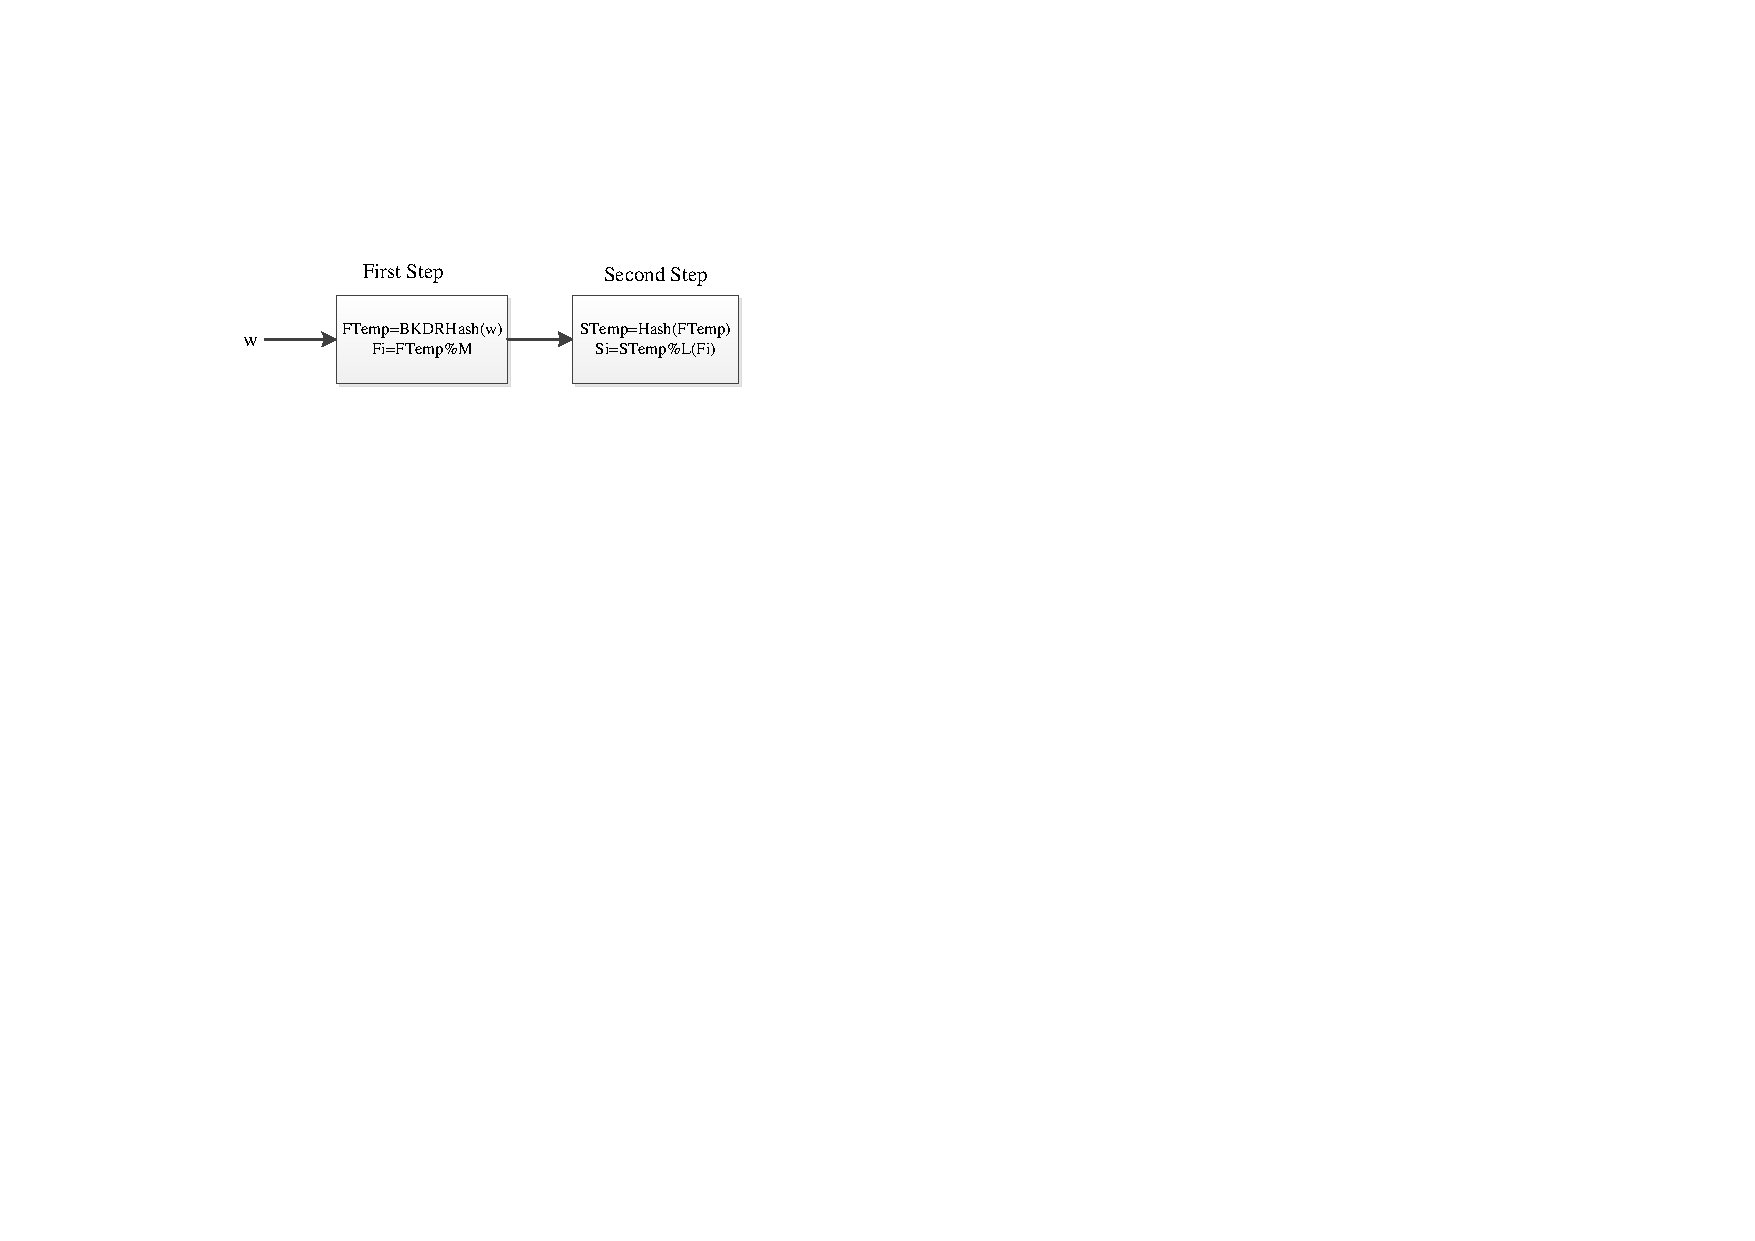
\includegraphics[width=3.5in,height=0.6in]{HASH}
\caption{The Hash Function} \label{F20}
\end{figure}

As illustrated in Fig. \ref{F20}, we determine the index of an entry in two steps. In the first step, we first map the keyword w of entry to the FTemp with the string hash function BKDRHash. It's worth to note that, although we apply BKDRHash as hash function, others string hash function can also be applied. And then, we obtain the $Fi$ by performing a modulus on FTemp with first-level index length M. In the second step, we hash the FTemp with an integer hash function and then perform a modulus on STemp with second-level index length of $Fi$ to get $Si$. After these two steps, each KHT entry has an index $(Fi,Si)$. Note that, a delicate situation arises when two or more entries share the same index $(Fi,Si)$ whose probability less than 0.5, which is demonstrated in \cite{cormen2001introduction}. In this case, \textbf{\textit{``linear probing''}} technique is utilized to tackle this problem. From Table \ref{T4} we know that there is a conflict situation between ``forest'' and ``shore''. As illustrated in Fig. \ref{F1}, when we try to insert the entry $e_4$ into KHT, $e_2$ has already stayed in location $(6,1)$. Due to location $(6,2)$ is occupied as well, with ``linear probing'', $e_4$ is inserted into $(6,3)$ ultimately, just as the solid arrow shown.

With KHT, for a specific query q we can retrieve the $RO_q$ in nearly $\Theta(|q.\omega|)$, and prune the unnecessary visits hugely.

\subsection{The Exact Algorithm MergeList}
For many real application scenarios, the number of query keywords submitted by users is limited. Motivated by this observation, we devise an exact algorithm MergeList in this section.

The straightforward method for the exact algorithm is to enumerate all the subsets of $RO_q$ and return the subset, which covers the query keywords not less than a given threshold and with minimum cost, as our optimal solution. This yields an exponential time complexity in terms of the number of objects in $RO_q$.

To further prune the search space, we delve into several efficient pruning strategies below.

Firstly, we sort the objects of $RO_q$ in ascending order of the cost distance. And we record the current optimal solution and its cost with notations $COS$ and $minCost$. Instead of enumerating all the subsets of $RO_q$ randomly, we construct the candidate subsets whose cost less than minCost by adding object into existing candidate subsets progressively.

\begin{lem}
    Given a sorted $RO_q$ which in ascending order of the cost distance. If for each existing candidate set \textbf{ecs}, the cost sum of ecs and the current visitorial object \textbf{cvo} in $RO_q$ is not less than minCost, then COS is the optimal solution.
    \begin{pot}
        Since $RO_q$ is sorted in ascending order of the cost distance. We know that each object behind cvo in $RO_q$ has a higher cost than cvo. If the cost sum of any ecs and cvo is not less than minCost, we can conclude that any ecs can not be the optimal solution, so we can terminate our procedure immediately.
    \end{pot}
\end{lem} \label{L5}

Secondly, there is an \textbf{\textit{``Apriori property''}} in the data mining field. \textbf{\textit{``All nonempty subsets of a frequent itemset must also be frequent''}}. In the sequel, we present a similar pruning strategy.

\begin{lem}
    If the cost sum of an ecs and cvo larger than the minCost, we can prune the ecs safely and any superset of it needs not to be computed.
    \begin{pot}
        If the cost sum of an ecs and cvo larger than the minCost, we know that ecs cannot be the optimal solution and any superset of ecs neither can be the optimal solution as well, so we can prune them safely.
    \end{pot}
\end{lem} \label{L6}

Further, only if G is a feasible solution, we can filter out any superset G', since G is superior to G' anyway.

In a word, Lemma 3 allows us to terminate the procedure earlier and Lemma 4 provides significant pruning ability. We elaborate the MergeList in Algorithm \ref{A4}.

The MergeList algorithm can be summarized as following three steps.
\begin{itemize}
    \item Step 1 (Construct $RO_q$): In this step, we construct the $RO_q$ and sort it in ascending order of cost distance.
    \item Step 2 (Add o into $ecs$): For object o in $RO_q$, we verify for each ecs whether delete it from candidate sets $SS$ or combine it with o and put it into $SS$.
    \item Step 3 (Iterative step): Repeat Step 2, until the terminal condition in Lemma 3 is met.
\end{itemize}

%The MergeList algorithm
\IncMargin{1em}
\begin{algorithm}[!hb]
\caption{$MergeList$} \label{A4}   % 给算法一个标签,以便其它地方引用该算法
%\DontPrintSemicolon
\SetKwInOut{Input}{Input}\SetKwInOut{Output}{Output}
\Input {The $KHT$ and the query $q$.}
\Output{A group $G$ of objects as resulting solution.}
\BlankLine
\LinesNumbered
$COS \longleftarrow \emptyset$\;
$SS \longleftarrow \emptyset$\;
$minCost \longleftarrow$ INFINITE\_MAX\;
$RO_q \longleftarrow$ compute the relevant object set to query q with $KHT$\;
sort $RO_q$ in ascending order of weight distance cost\;
put empty set ${\O}$ into SS\;
\For{each object $o \in RO_q$} {
    \If{$wd(o,q)\geq minCost$} {
        break\;
    }
    \For{each $ecs \in SS$}{
        \If{the cost sum of $ecs$ and $o$ not less than $minCost$} {
            delete $ecs$ from $SS$\;
            continue\;
        }
        $tempSet \longleftarrow ecs\cup \{o\}$\;
        \eIf{$tempSet$ is a feasible solution} {
            $COS \longleftarrow tempSet$\;
            $minCost \longleftarrow$ the cost of $tempSet$\;
            delete $ecs$ from $SS$\;
        } {
            put $tempSet$ into SS\;
        }
    }
    \If{$SS == {\O}$} {
        break\;
    }
}
$G \longleftarrow COS$\;
return $G$ as the final solution\;
\end{algorithm}
\DecMargin{1em}

As discussed above, in MergeList algorithm, we construct the candidate set by adding the object into ecs progressively. We use $SS$ to store the ecs, and initiate $SS$ with the empty set (line 6). For each object o in $RO_q$, if the cost of o not less than minCost then we terminate our procedure (lines 8-9). Otherwise, for each ecs satisfies Lemma 4, we prune it directly (lines 11-13). If $tempSet$ is a feasible solution, we use it to update the $COS$ and $minCost$ (lines 15-18), otherwise we add it into $SS$.

%\begin{table}[h]
%\centering
%\begin{tabular}{|c|c|c|c|c|c|}
%\hline
% OID & $o_1$ & $o_2$ & $o_3$ & $o_4$ & $o_5$\\
%\hline
 %Cost Distance to q& 2 & 2.5 & 4 & 5 & 7 \\
%\hline
% CP &0.1, 0.0&0.1, 0.3&0.3, 0.1&0, 0.3&0.1, 0.3\\
%\hline
%\end{tabular}
%\caption{An example of MergeList} \label{T6}
%\end{table}
\begin{figure}[!ht] \centering
    \subfigure[] { \label{MergeList-Q}
    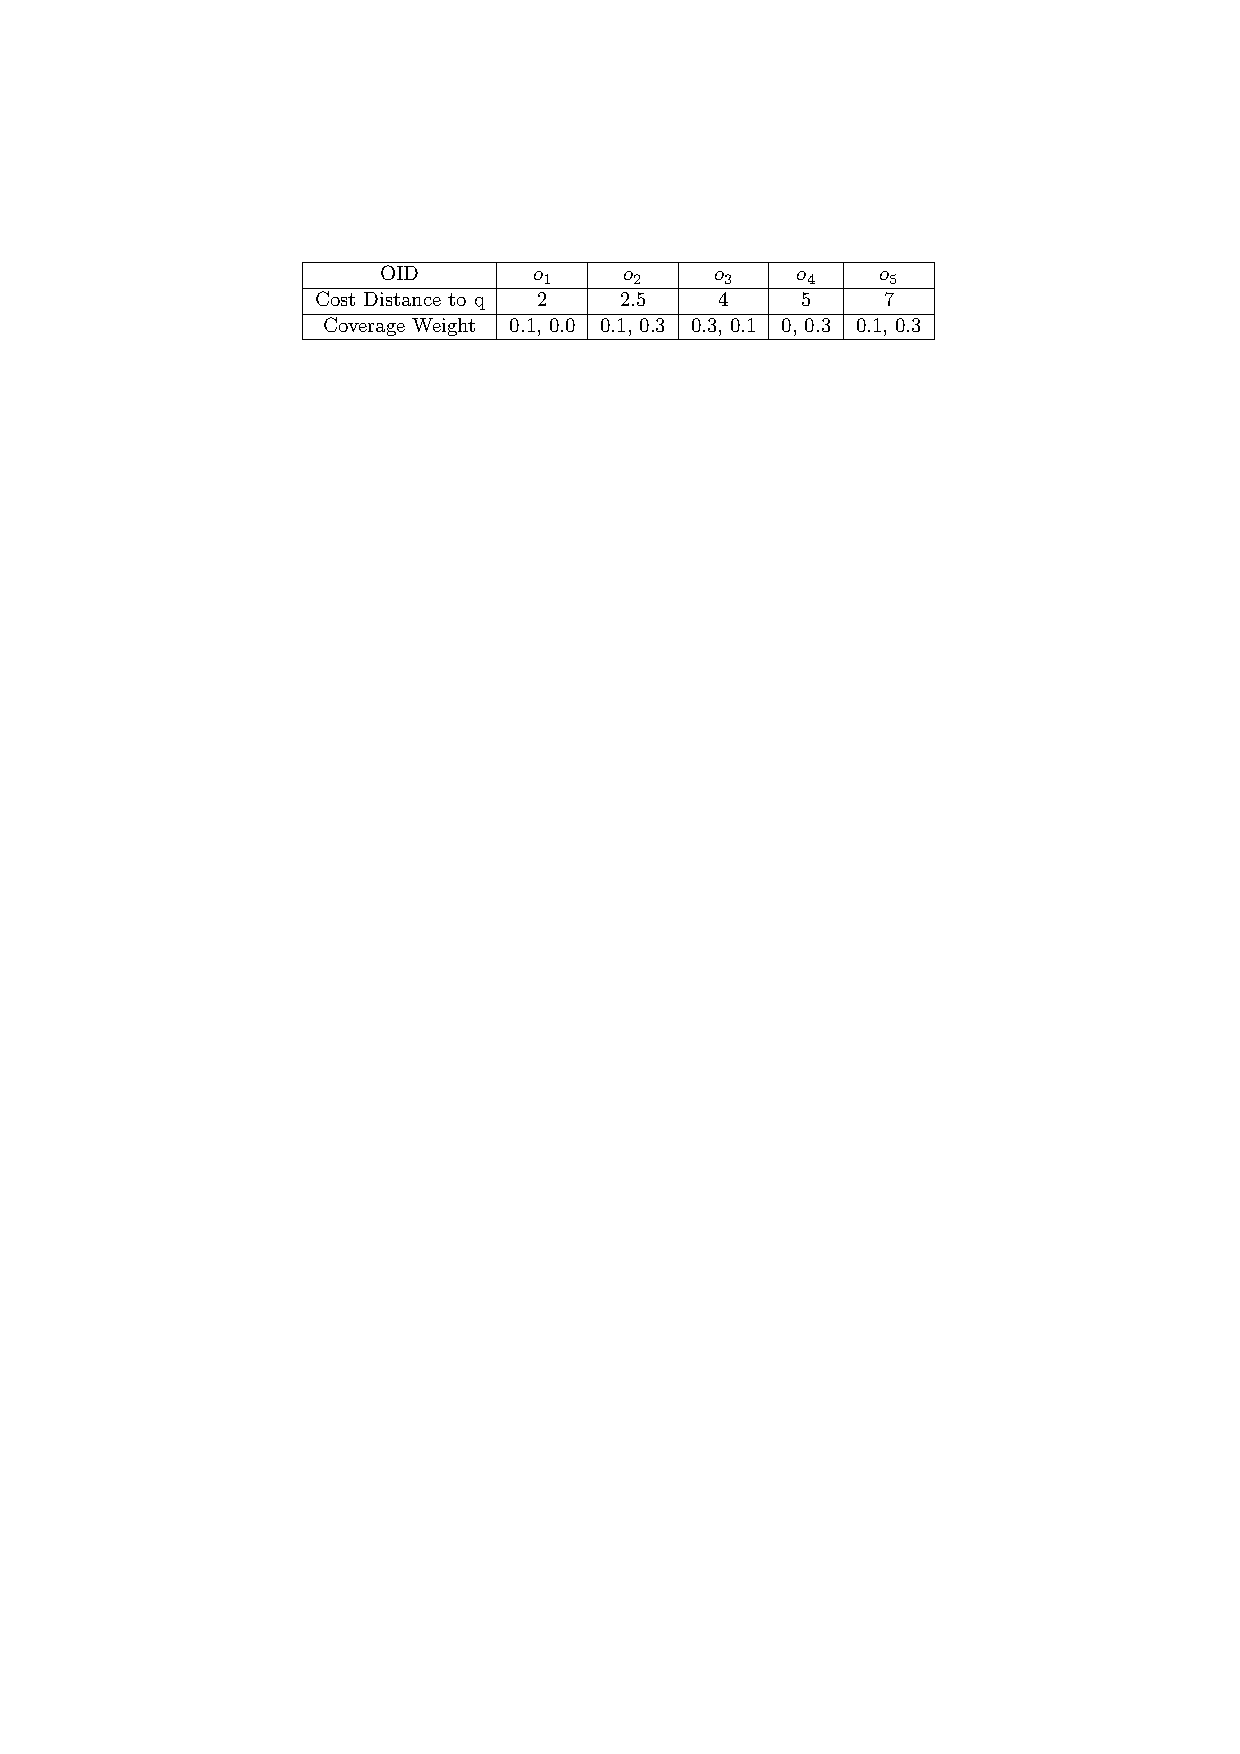
\includegraphics[width=3in,height=0.5in]{MergeList-Q}
    }
    \subfigure[] { \label{MergeList-S}
    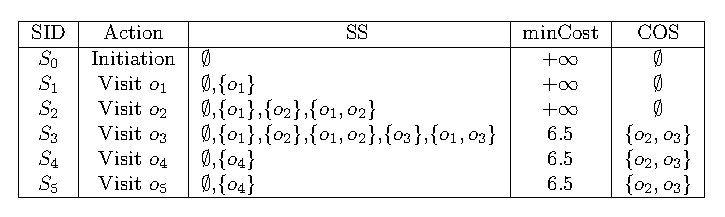
\includegraphics[width=3in,height=1.2in]{MergeList-S}
    }
\caption{An example of MergeList}
\label{F30}
\end{figure}

\textbf{Example 3}: Consider a query q with two keywords $q.\omega=\{\lambda_1, \lambda_2\}$. Fig. \ref{F30}a illustrates the $RO_q$ and the cost distance to q and the corresponding coverage weight. We illustrate the process of MergeList in Fig. \ref{F30}b. There are total six steps to answer this query.
\begin{itemize}
    \item Step 1 (Initiation): We initiate the $SS$, $minCost$ and $COS$ in this step.
    \item Step 2 (Visit $o_1$): Due to $RO_q$ in Fig. \ref{F30}a has been sorted, we visit the object according to the order in Fig. \ref{F30}a We first visit $o_1$, and merge it with ecs in $SS$.
    \item Step 3 (Visit $o_2$): Object $o_2$ is merged with ecs in $SS$.
    \item Step 4 (Visit $o_3$): In this step, we obtain a feasible solution $COS=\{o_2,o_3\}$. And to filter candidate sets with Lemma 4.
    \item Step 5 (Visit $o_4$): In this step, ecs which satisfies Lemma 4 is pruned by COS.
    \item Step 6 (Visit $o_5$): Because the cost of $o_7$ is larger than $minCost$, so Lemma 3 is met and COS is the optimal solution.
\end{itemize}

%\begin{table}[h]
%\centering
%\begin{tabular}{|c|c|p{2cm}|c|c|}
%\hline
% SID & Action & SS & minCost & COS\\
%\hline
%$S_0$ & Initiation & $\emptyset$ & $+\infty$ & $\emptyset$\\
%$S_1$ & Visit $o_1$ & $\emptyset$,\{$o_1$\} & $+\infty$ & $\emptyset$\\
%$S_2$ & Visit $o_2$ & $\emptyset$,\{$o_1$\},\{$o_2$\},\{$o_1,o_2$\} & $+\infty$ & $\emptyset$\\
%$S_3$ & Visit $o_3$ & $\emptyset$,\{$o_1$\},\{$o_2$\},\{$o_1,o_2$\},\{$o_3$\},\{$o_1,o_3$\} & 6.5 & \{$o_2,o_3$\}\\
%$S_4$ & Visit $o_4$ & $\emptyset$,\{$o_4$\} & 6.5 & \{$o_2,o_3$\}\\
%$S_5$ & Visit $o_5$ & $\emptyset$,\{$o_4$\} & 6.5 & \{$o_2,o_3$\}\\
%\hline
%\end{tabular}
%\caption{The process of MergeList} \label{T7}
%\end{table}

\begin{thm}
    (Correctness of MergeList): The MergeList algorithm always produce the correct result set.
    \begin{pot}
        Assuming the number of objects in $RO_q$ is n, hence, there are up to $2^n-1$ candidate sets. Each ecs either used to update the $COS$ or pruned by the $COS$. If the cost of ecs less than $minCost$, we take ecs as our $COS$. Otherwise, we prune ecs and any superset of it. Hence, it is suffice to show that MergeList never prune any feasible solution whose cost less than $minCost$ (false negatives), and never maintain the ecs whose cost larger than $minCost$ (false positives). So the MergeList algorithm always produce the correct result.
    \end{pot}
\end{thm}













\section{Algorithms}
%ALGORITHM
Considering the inherent complexity of NP-hard problem, we design two approximation algorithms, namely CubeTree and MaxMargin with provable approximation ratio in Sections 5.1 and 5.2 respectively. Besides, we also propose the exact algorithm MergeList in Section 5.3.

\subsection{Approximation Algorithm MaxMargin}
In section 5.1 we show how to utilize the CubeTree algorithm to handle our problem. Although CubeTree can solve our problem with provable approximation ratio, however, as presented in Theorem 2, the approximation ratio of CubeTree is unstable due to the relevance with final solution. In this section, we elaborate the MaxMargin algorithm, which is inspired by the greedy strategy adopted by the WSC problem \cite{chvatal1979greedy}, which with more stable performance in terms of approximation ratio. To address WSC problem, the greedy strategy iteratively selects the current optimal subset and updates subsets that have not been visited yet accordingly. We modify this strategy by iteratively selecting the object with maximum $cr(o,q)$, and updating objects that have not been visited for our problem. The naive version of MaxMargin solves the problem by four steps. We use G to reserve the solution.
\begin{itemize}
    \item Step 1 (Construct the $RO_q$): Construct the relevant set $RO_q$ with KHT and sort the objects of $RO_q$ in descending order of $cr(o,q)$.
    \item Step 2 (Select the optimal object): In this step, MaxMargin adds the current optimal object o with maximum $cr(o,q)$ into G. Then, o is deleted from $RO_q$.
    \item Step 3 (Update $RO_q$): After adding o into G, we update the $cr(o,q)$ of remaining objects in $RO_q$.
    \item Step 4 (Iterative step): Repeat Step 2 and Step 3 until the weight constraint in definition 4 is satisfied. Then we take G as our final solution.
\end{itemize}

Obviously, two major drawbacks degrade the performance of naive version: 1) lacking of efficient pruning strategies; 2) updating all the remaining objects for each iteration in Step 3 is time consuming. To further boost the search efficiency, we take a look at several notions which settle aforementioned drawbacks collectively.

\begin{definition}
    \textbf{(Keyword Max Priority Queue).}: For a given keyword $\lambda$, we define the Keyword Max Priority Queue (KMPQ) of $\lambda$ as the max priority queue of $RO_\lambda$ according to the value of $cr(o,q)$.
\end{definition}

Each element of KMPQ of the form $(nid,oid,cr,cv)$, where nid and oid correspond to the identifier of element and the object, respectively. $cr$ represents the contribution ratio of oid and cv is a $|q.\omega|$ dimensions vector to record the $cw(o,\lambda)$ for each keyword in $q.\omega$. Instead of constructing the $RO_q$, we construct the KMPQ for each query keyword. Once $cov(G,\lambda)$ reaches $q.\theta$, we can prune objects in the KMPQ of $\lambda$ safely, which significantly exalts the performance.

To address the second drawback, we expand the notion of contribution ratio to fit in with our algorithm.

\begin{definition}
    \textbf{(Dynamic contribution ratio).}: Given a query q and an object o, we define the dynamic contribution ratio (dcr) of object o in iteration r as follows:
    \begin{equation}
        dcr_{q}^{r}(o)=\frac{cov^r(o,q)}{cd(o,q)}
    \end{equation}
\end{definition}

Note that the major difference between $dcr_{q}^{r}(o)$ and $cr(o,q)$ is that, we replace $cov(o,q)$ with $cov^r(o,q)$, where $cov^r(o,q)$ denotes the last contribution ratio of o after $r$th object added into result set. We do not update $dcr$ for object o in each iteration r until o is chosen as the current optimal object.

\begin{lem}
    Given a query q, an object o, two integers m, n and $m \leq n$, then $dcr_{q}^{n}(o)\leq dcr_{q}^{m}(o)$.
    \begin{pot}
        After each iteration r, the value of $cov^r(o,q)$ is comparable or below than the former iteration. Besides, $cd(o,q)$ is constant in each iteration, which results in the decreasing of $dcr^{r}_{q}(o)$. If $m\leq n$, we can safely draw the conclusion that the $dcr_{q}^{n}(o)$ is not larger than $dcr_{q}^{m}(o)$.
    \end{pot}
\end{lem} \label{L2}

Instead of updating all the remaining objects after each iteration, we update the object until it is chosen as the optimal object. Lemma 2 indicates that we can always choose the newly updated object with maximum $dcr^{r}_{q}(o)$ as current optimal object, and objects whose $dcr$ less than $dcr^{r}_{q}(o)$ unnecessary to be updated, which significantly prunes the updating overhead.

We summarize the aforementioned discussion by following three steps to improve the naive version. And we use G to reserve the final solution and RV to record the residuals.
\begin{itemize}
    \item Step 1 (Construct the KMPQ): In this step, we construct the KMPQ for each keyword of $q.\omega$.
    \item Step 2 (Select the optimal object): Select the current optimal object o from all the KMPQs. If o already in G, then continue to select next optimal object. Otherwise, we add o into G if $cov^r(o,q)$ less than RV in all dimensions. Otherwise, we update the $cr(o,q)$ of o and reinsert it into KMPQ.
    \item Step 3 (Iterative step): Repeat Step 2 until RV equals to 0 in all dimensions. Then we take G as our final solution.
\end{itemize}

Algorithm \ref{A3} illustrates the details of MaxMargin algorithm.
%MaxMargin algorithm
\IncMargin{1em}
\begin{algorithm}[!htb]
\caption{$MaxMargin$} \label{A3}   % ���㷨һ����ǩ���Ա������ط����ø��㷨
%\DontPrintSemicolon
\SetKwData{G}{G}\SetKwData{RV}{RV}\SetKwData{indicator}{indicator}
\SetKwData{PQ}{PQ} \SetKwData{maxMargin}{maxMargin}
\SetKwInOut{Input}{Input}\SetKwInOut{Output}{Output}
\Input {The $KHT$ and the query $q$.}
\Output{A group $G$ of objects as approximation solution.}
\BlankLine
\LinesNumbered
\G$\longleftarrow \emptyset$; \maxMargin $\longleftarrow 0.0$; \indicator $\longleftarrow -1$\;
\For{$i \longleftarrow 0$ \KwTo $|q.\omega|-1$} {
    $RV[i] \longleftarrow q.\theta$\;
    construct the KMPQ $PQ[i]$ for $q.\omega[i]$ with $KHT$\;
}
$r \longleftarrow 0$\;
\While{exists a dimension i satisfies $RV[i]>0.0$} {
    \For{each valid $PQ[j] \in PQ$} {
        $o \longleftarrow PQ[j].top()$\;
        \If{$dcr_q^r(o)>maxMargin$} {
            $maxMargin \longleftarrow dcr_q^r(o)$\;
            $indicator \longleftarrow j$\;
            $maxOID \longleftarrow o$\;
        }
    }
    \If{$maxOID \in G$} {
        $PQ[indicator].dequeue()$\;
        continue\;
    }
    \eIf{all dimensions satisfy $maxOID.cv[i]<RV[i]$} {
        \G $\longleftarrow G\cup \{maxOID\}$\;
        \For{$j \longleftarrow 0$ \KwTo $|q.\omega|-1$} {
            \eIf{$RV[j]\geq maxOID.cv[j]$} {
                $RV[j] \longleftarrow RV[j]-maxOID.cv[j]$\;
            } {
                $RV[j] \longleftarrow 0$\;
                set the $PQ[j]$ to be invalid\;
            }
        }
        $PQ[indicator].dequeue()$\;
        r++\;
    } {
        \For{$j \longleftarrow 0$ \KwTo $|q.\omega|-1$} {
            \If{$RV[j]< maxOID.cv[j]$} {
                $maxOID.cv[j] \longleftarrow RV[j]$\;
            }
        }
        recompute the $dcr_q^r(maxOID)$\;
        $PQ[indicator].dequeue()$\;
        $PQ[indicator].enqueue(maxOID)$\;
    }
}
return $G$ as the final solution\;
\end{algorithm}
\DecMargin{1em}

 MaxMargin utilizes the residual vector RV to record the difference between $q.\theta$ and the coverage weight of G for each query keyword dynamically. Initially, each dimension of RV is set to be $q.\theta$ (line 3). There are two different cases when processing the selected optimal object in each iteration. Case 1: If all dimensions satisfy $maxOID.cv[i]<RV[i]$ (lines 16-25), it needs not to update maxOID and we update RV accordingly. Case 2: Otherwise, we update the dcr of $maxOID$ and the PQ[indicator]. Algorithm terminates until RV equals to 0. Note that, in Algorithm \ref{A3}, we set $PQ[j]$ to invalid if $RV[j]$ is 0 (line 23). Put differently, we prune all the objects in $PQ[j]$ once the $cov(G,q.\omega[j])$ reaches the threshold $q.\theta$. What's more, we update the object $maxOID$ (lines 27-32) only when the coverage weight of o larger than RV in some dimensions instead of updating the remaining $RO_q$ in naive version. Both of these two strategies significantly improve the performance of MaxMargin algorithm.

\begin{figure}
\centering
\includegraphics[width=3.5in, height=3.5in]{maxMargin}
\caption{KMPQ of query q in Table \ref{T2}}
\label{F3}
\end{figure}

\textbf{Example 2}: Let's go back to the KaGWC query q depicted in Table \ref{T2}. As illustrated in Fig. \ref{F3}, we answer the query q in four steps, as follows.
\begin{itemize}
    \item Step 1 (Initial state): In this step, we construct the KMPQ for ``mountain'' and ``temple'', and initiate the $RV=\{0.4,0.4\}$ and $G=\emptyset$ as depicted in Figs. \ref{F3}a and \ref{F3}b.
    \item Step 2 (Fetch $o_3$): Due to the two KMPQs have common optimal object $o_3$, we can select $o_3$ from any of these two KMPQs. And we select $o_3$ from ``mountain''. After fetching $o_3$ from ``moutain'', the KMPQ of ``moutain'' is reorganized and the RV and G are updated as Fig. \ref{F3}c.
    \item Step 3 (Delete $o_3$): As depicted in Figs. \ref{F3}c and \ref{F3}d. After fetching $o_3$, the current optimal object is $o_3$ of ``temple''. However, $o_3$ has been in G. So we delete it from ``temple'' directly, as illustrated in Fig. \ref{F3}f.
    \item Step 4 (Fetch $o_1$): Again, the two KMPQs have common optimal object. We select $o_1$ from ``mountain'', and put it into G. Up to now, RV is equal to 0. We terminate our procedure and return G as the final solution.
\end{itemize}

\begin{thm}
    The approximation ratio of MaxMargin is not larger than $\frac{H(\lfloor cov+1\rfloor)}{q.\theta}$, where $cov$ is the largest $cov(o_j,q)$ for all $o_j \in RO_q$.
    \begin{pot}
        Inspired by the proof in \cite{chvatal1979greedy}, we provide the approximation ratio proof of MaxMargin here. We use m, n to denote the number of elements in $|q.\omega|$ and $|RO_q|$ respectively. We define a $m\times n$ matrix $P=(p_{ij})$ by
        \begin{displaymath}
            p_{ij} = \left \{
                \begin{array}{ll}
                    cw(o_j,q.\omega[i]) & \textrm{if $q.\omega[i] \in o_j.\omega$,}\\
                    0 & \textrm{otherwise.}\\
                \end{array} \right.
        \end{displaymath}

        According to the definition of P, we know that the n columns of P is n coverage weight vectors of n objects. The goal of MaxMargin is to retrieve a group G of objects. And we utilize the incidence vector $x=(x_j)$ to denote the cover set. Clearly, the incidence vector x of an arbitrary cover satisfies:

        \begin{eqnarray*}
            \sum_{j=1}^n p_{ij}x_j \geq q.\theta & for\ all\ i, \\
             x_j \in \{0,1\}  & for \ all \ j.\\
        \end{eqnarray*}

        For ease of presentation, in the following, we refer to the cost distance of $o_j$ as $c_j$. And we claim that these inequations imply
        \begin{equation} \label{E6}
            \sum_{j=1}^{n} H(\lfloor cov_j^1+1\rfloor)c_j x_j\geq q.\theta \sum(c_j: where\ o_j \in G)
        \end{equation}
        for the cover G returned by the greedy heuristic. Once (\ref{E6}) is proved, the theorem will follow by letting x be the incidence vector of an optimal cover.

        To prove (\ref{E6}), it will suffice to exhibit nonnegative numbers $y_1, y_2, ..., y_m$ such that
         \begin{equation} \label{E7}
            \sum_{i=1}^{m}p_{ij}y_{i} \leq H(\sum_{i=1}^{m}p_{ij})c_{j} \quad for\ all\ j
        \end{equation}
        and such that
         \begin{equation} \label{E8}
            \sum_{i=1}^{m} y_{i} = \sum(c_j: where\ o_j \in G)
        \end{equation}
        for then
        \begin{eqnarray*}
            \sum_{j=1}^n H(\sum_{i=1}^m p_{ij})c_j x_j &\geq& \sum_{j=1}^n (\sum_{i=1}^m p_{ij} y_i)x_j\\
            &=& \sum_{i=1}^m(\sum_{j=1}^n p_{ij}x_j)y_i \\
            &\geq& q.\theta \sum_{i=1}^m y_i\\
            &=& q.\theta \sum(c_j: where\ o_j \in G)\\
        \end{eqnarray*}
        as desired.

        The numbers $y_1, y_2, ..., y_m$ satisfying (\ref{E7}) and (\ref{E8}) have a simple intuitive interpretation: each $y_i$ can be interpreted as the cost paid by MaxMargin for covering the keyword $q.\omega[i]$. We use $cov_{j}^{r}$ to denote the coverage weight of query q covered by object $o_j$ at the beginning of iteration r. Without loss of generality, we may assume that G is \{$o_1$,$o_2$,...,$o_r$\}  after r iteration, and so
        \begin{displaymath}
            \frac{cov_{r}^{r}}{c_r} \geq \frac{cov_{j}^{r}}{c_j}
        \end{displaymath}
        for all r and j. If there are t iterations altogether then
        \begin{displaymath}
            \sum(c_j: j \in G)=\sum_{j=1}^{t}c_{j},
        \end{displaymath}
        and
        \begin{displaymath}
            y_{i}=\sum_{r=1}^{t}\frac{c_{r}\cdot cw(o_r, q.\omega[i])}{cov_{r}^{r}}.
        \end{displaymath}
        We know that
        \begin{displaymath}
            \sum_{i=1}^{m}y_i=\sum_{i=1}^{m}\sum_{r=1}^{t}\frac{c_{r}\cdot cw(o_r,  q.\omega[i])}{cov_{r}^{r}}=\sum_{r=1}^{t}c_{r}
        \end{displaymath}

        For any $o_j$ in $RO_q$, we know that the $cov_{j}^{r}$ decrease as the iteration continues. We assume s is the largest superscript such that $cov_{j}^{s}>0$ then
        %\begin{flushleft}
        \begin{eqnarray*}
            \sum_{i=1}^{m}p_{ij}y_{i}&=&\sum_{r=1}^{s}(cov_j^r-cov_j^{r+1})\cdot \frac{c_r}{cov_r^r}\\
            &\leq& c_j\sum_{r=1}^{s}\frac{cov_j^r-cov_j^{r+1}}{cov_j^r}\\
            &=&c_j\sum_{r=1}^s\frac{cov_j^r-cov_j^{r+1}}{cov_j^r}\\
            &\leq& c_j\sum_{r=1}^s\frac{\lfloor cov_j^r + 1\rfloor - \lfloor cov_j^{r+1}\rfloor}{\lfloor cov_j^r + 1\rfloor} \\
            &=&c_j\sum_{r=1}^s \sum_{l=\lfloor cov_j^{r+1} +1\rfloor}^{\lfloor cov_j^r +1\rfloor} \frac{1}{cov_j^r}\\
            &\leq& c_j\sum_{r=1}^s \sum_{l=\lfloor cov_j^{r+1} +1\rfloor}^{\lfloor cov_j^r +1\rfloor} \frac{1}{l}\\
            &=&c_jH(\lfloor cov_j^1 +1\rfloor)-c_jH(\lfloor cov_j^s+1\rfloor)\\
            &\leq& c_jH(\lfloor cov_j^1+1\rfloor)\\
        \end{eqnarray*}
        %\end{flushleft}
    \end{pot}
\end{thm}



\section{Empirical Study}
%EMPIRICAL STUDY
In this section, we experimentally study the performance of our proposed algorithms through comprehensive experiments on both real and synthetic datasets. We describe the experimental settings in Section 6.1, and report the performance of our proposed algorithms for KaGWC queries on synthetic and real datasets in Sections 6.2 and 6.3 respectively.

\subsection{Experimental Setup}
\textbf{Algorithms.} We evaluate the performance of the following proposed algorithms: the approximation algorithm CubeTree in Section 5.1, the approximation algorithm MaxMargin in Section 5.2, and the exact algorithm MergeList in Section 5.3.

\textbf{Data and queries.} We conduct experiments with two datasets, namely synthetic dataset and real-life dataset. Our experiments were carried out primarily on synthetic dataset with five major factors, namely, 1) \textit{the total number of keywords in the spatial object database} (TK), 2) \textit{data size} (DS), 3) \textit{the number of query keywords} (QK), 4) \textit{the upper bound of the number of keywords associated with each object} (KD), not the fixed number of keywords in \cite{zhang2009keyword}, 5) \textit{the weight constraint threshold of query q} (TS). We study their effect on both response time and approximation ratio in three algorithms. Synthetic data generator generates three types of datasets following the uniform, random and zipf (URZ) distribution respectively. For each query, we repeat 5 times experiment for each type of dataset. We also included real dataset CA, which was collected from the U.S. Board on Geographic Names(geonames.usgs.gov). For each query, we repeat 10 times experiment.

All three algorithms were implemented in C/C++ and run on an Intel(R) Core(TM)2 Quad CPU Q8400 @2.66Hz with 4GB RAM.

\subsection{Results on Synthetic Dataset}
To measure the comprehensive performance of our algorithms on different types of datasets, in this section, we employ the URZ average response time $(URZA\_T)$ and URZ average approximation ratio $(URZA\_R)$ as the measurements, where $URZA\_T=\frac{T_u+T_r+T_z}{3}, URZA\_R=\frac{R_u+R_r+R_z}{3}$. $Tu, Tr, Tz$ and $Ru, Rr, Rz$ represent the response time and approximation ratio of uniform, random and zipf distribution datasets, respectively. Table \ref{T6} illustrates all the possible values for these factors in subsequent experiments. Note that, we use bold font to denote the default value for each factor. We repeat query 5 times for each dataset, and we take the average value of all datasets as the final result.

\begin{table}[h]
\centering
\begin{tabular}{|l|l|}
\hline
Factors & Instance Value \\
\hline
TK & 50,100,150,200,250,\textbf{300} \\
\hline
DS($10^4$) & 1,\textbf{10},30,50,70,90\\
\hline
QK & 2,\textbf{3},4,5,6,7,8,9 \\
\hline
KD & 3,5,\textbf{7},9,11,13,15 \\
\hline
TS & 0.1,\textbf{0.2},0.3,0.4,0.5,0.6,0.7 \\
\hline
\end{tabular}
\caption{The real data of CA}
\label{T6}
\end{table}

\begin{figure}[h] \centering
    \subfigure[] { \label{TKa}
    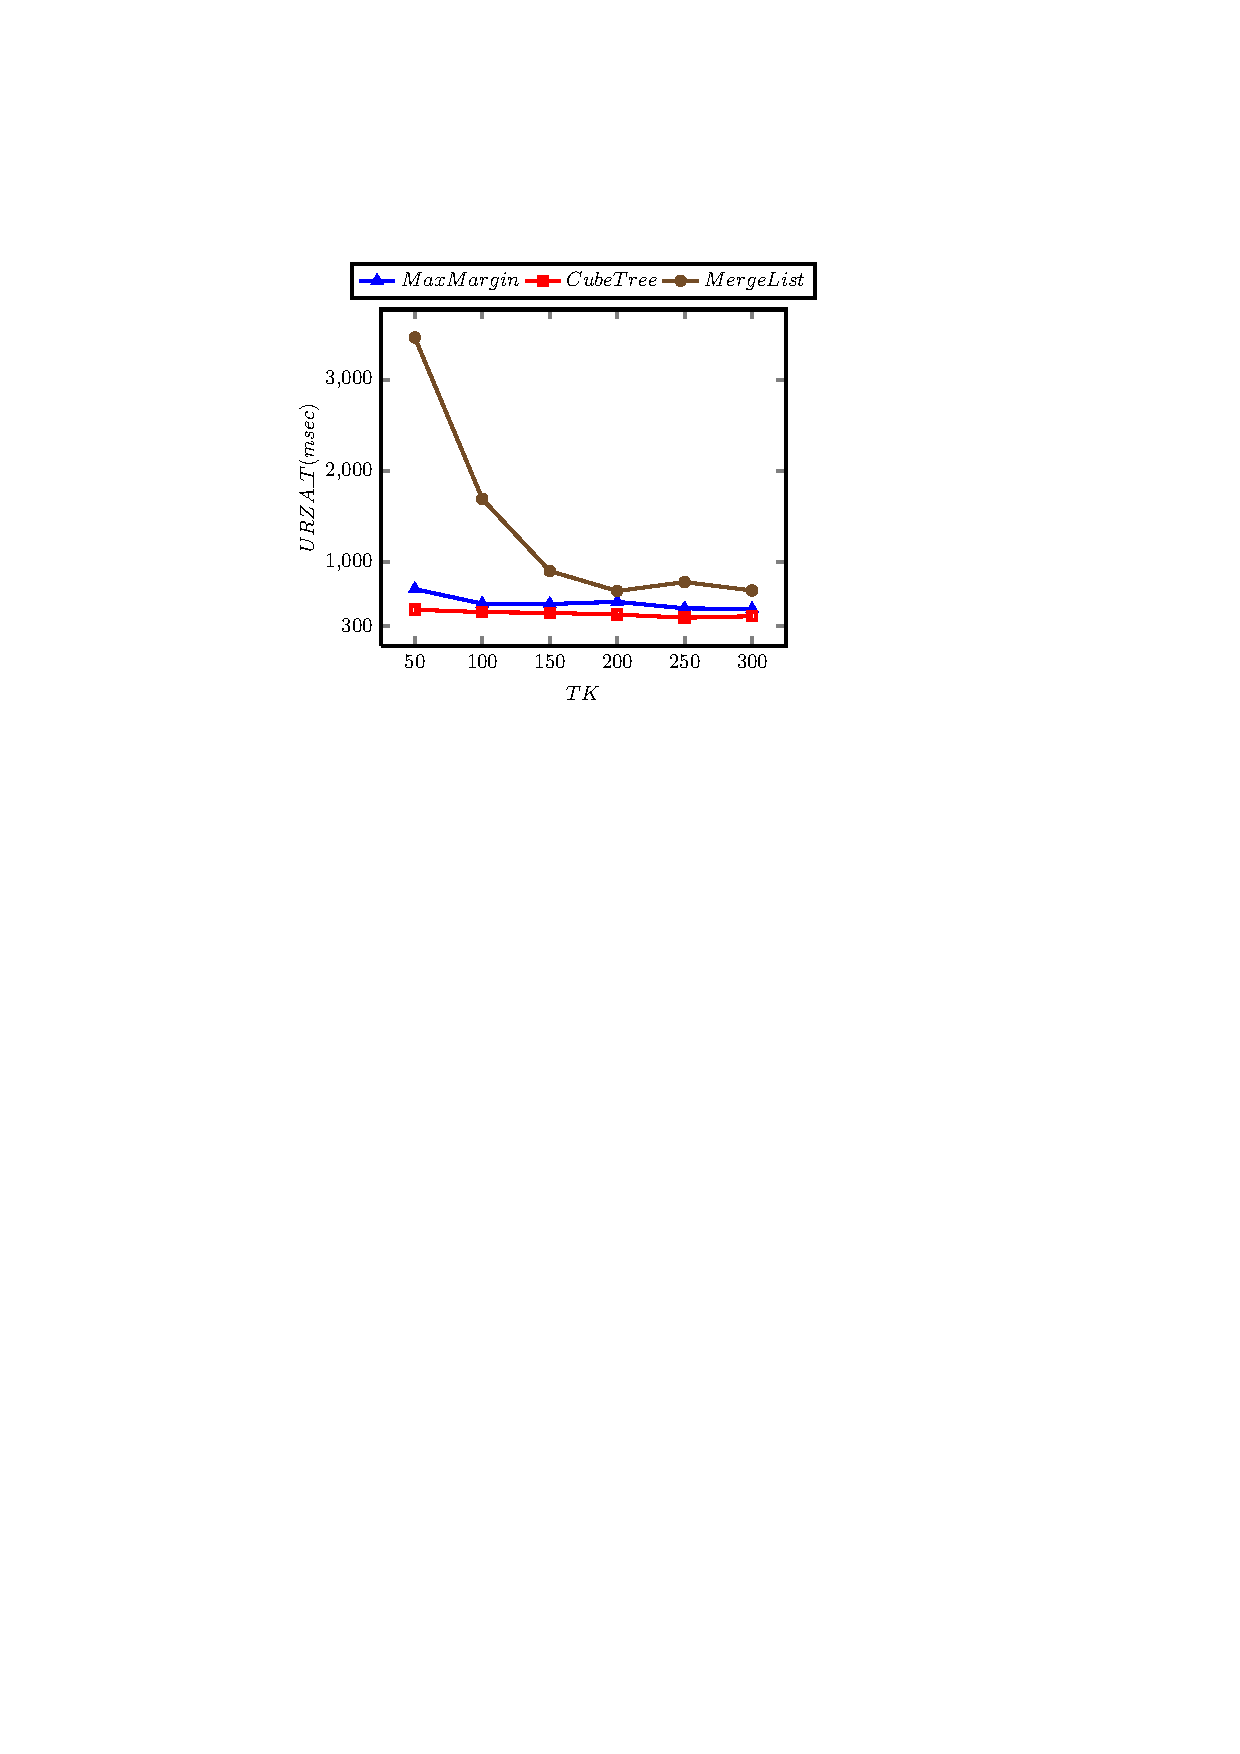
\includegraphics[width=1.5in,height=1.5in]{TK-T}
    }
    \subfigure[] { \label{TKb}
    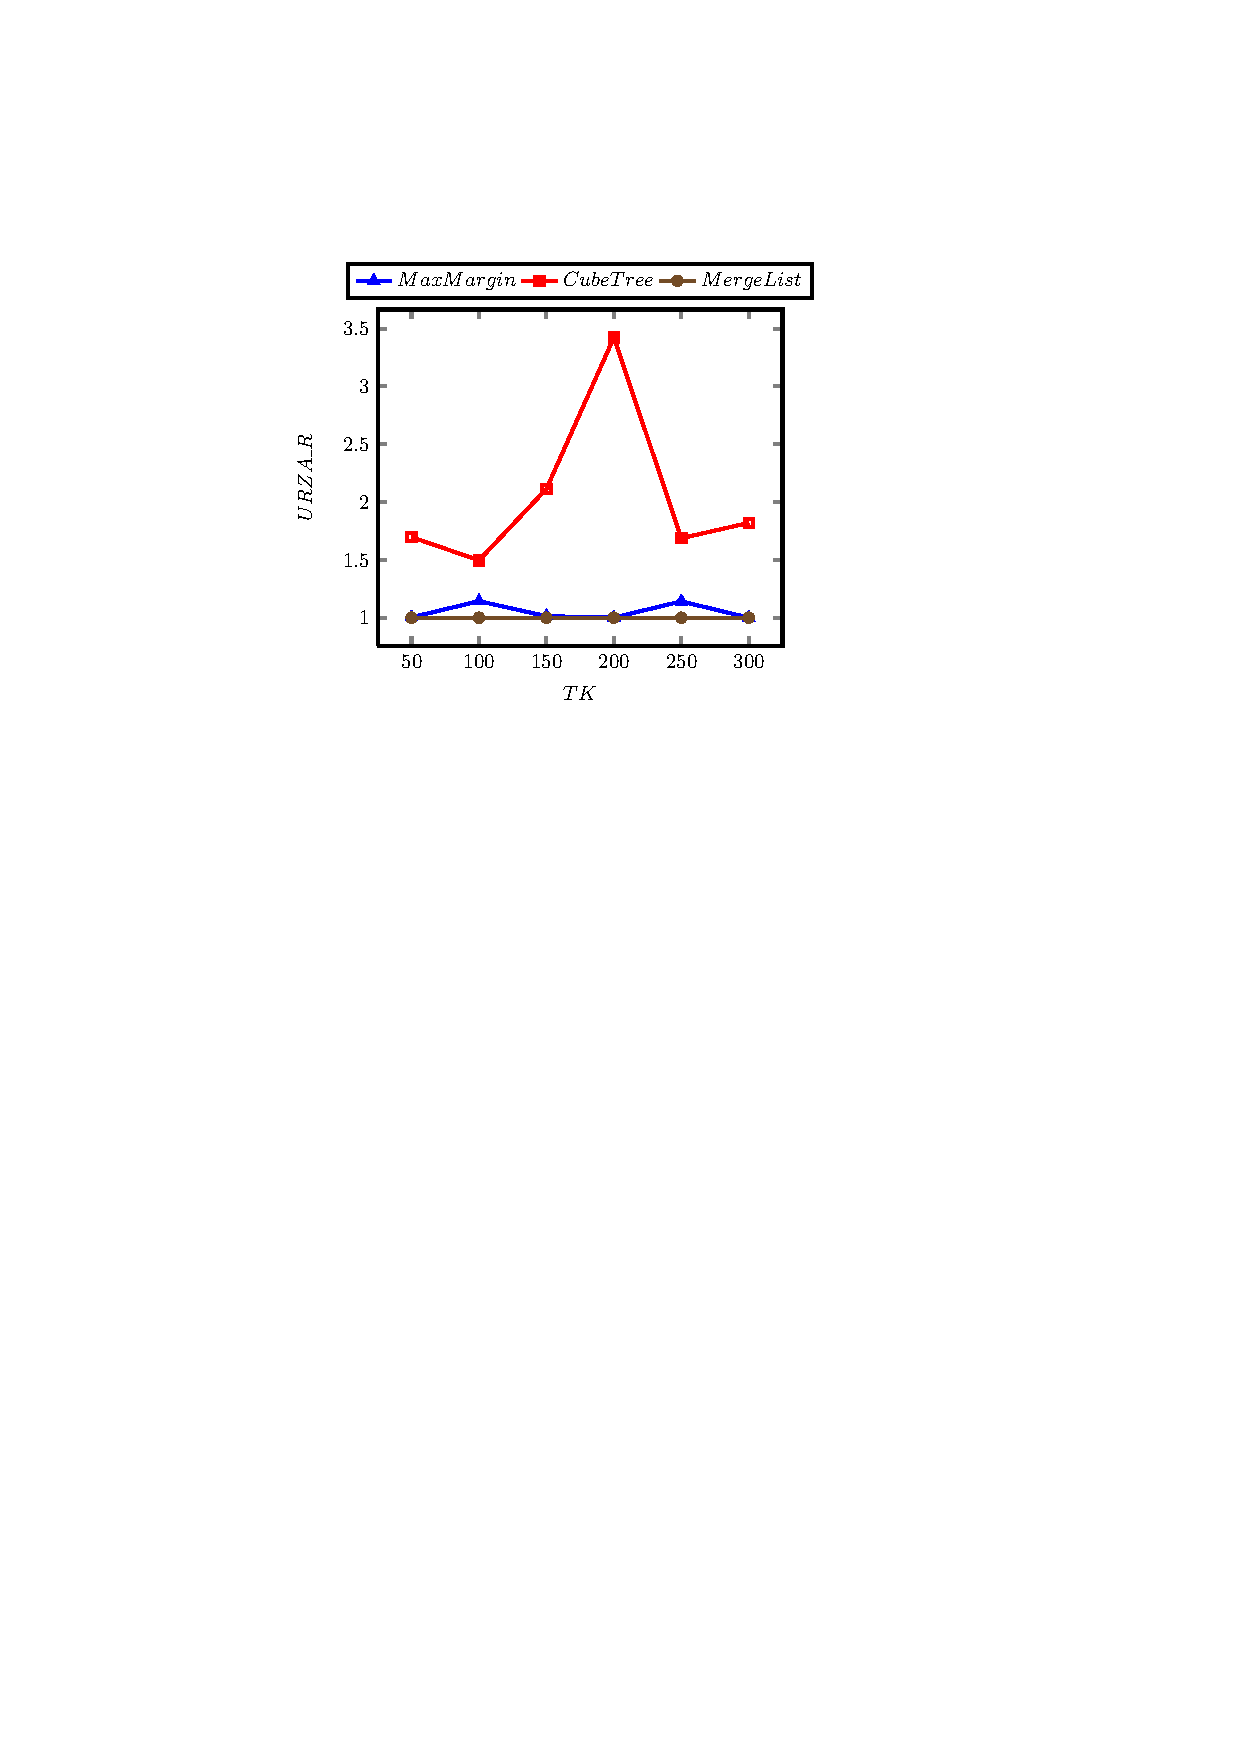
\includegraphics[width=1.5in,height=1.5in]{TK-R}
    }
\caption{Varying the factor TK}
\label{F4}
\end{figure}

\textbf{\textit{Varying the factor TK}}. Figs. \ref{F4}a and \ref{F4}b show the response time and approximation ratio of three algorithms respectively, when we vary the value of TK. As shown in Fig. \ref{F4}a, the response time of MergeList decreases dramatically as TK becomes larger. CubeTree runs faster than does MaxMargin. And both CubeTree and MaxMargin decrease slightly as TK is increased. The reason behind is that, when other factors are fixed, the larger the TK, the smaller number of relevant objects, and thus smaller objects need to be handled during algorithms execution. It is also denoted that MergeList is more sensitive than CubeTree and MaxMargin in terms of TK. In Fig. \ref{F4}b, we set the approximation ratio of the exact algorithm MergeList equals to 1, which is also adopted by the subsequent experiments. It can be observed from Fig. \ref{F4}b that, MaxMargin achieves a much better accuracy than CubeTree. And the approximation ratio of MaxMargin changes slightly and with an upper bound 1.25 when we vary the value of TK. In contrast, the approximation ratio of CubeTree changes dramatically and with an upper bound 3.5. This is because MaxMargin always select the optimal object and update the contribution ratio dynamically.

\begin{figure}[h] \centering
    \subfigure[] { \label{DSa}
    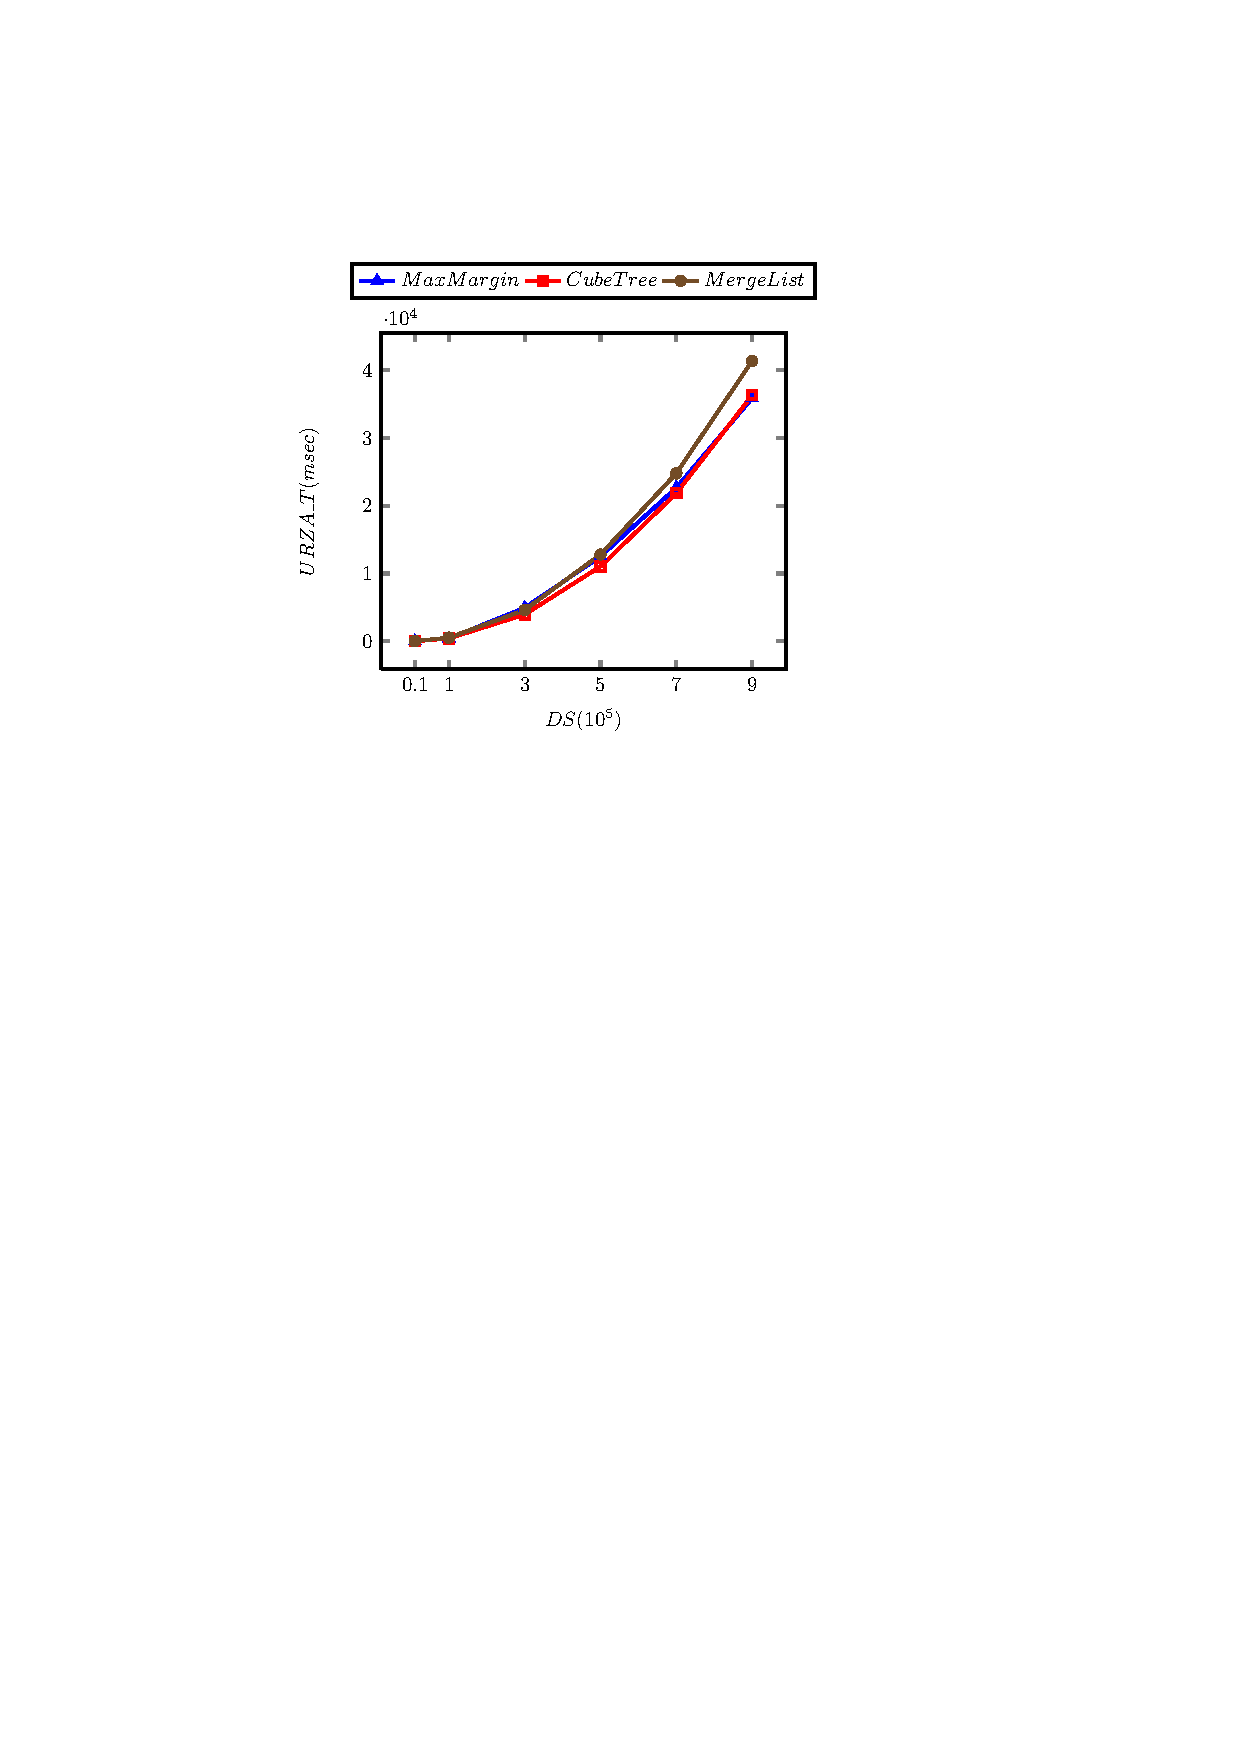
\includegraphics[width=1.5in,height=1.5in]{DS-T}
    }
    \subfigure[] { \label{DSb}
    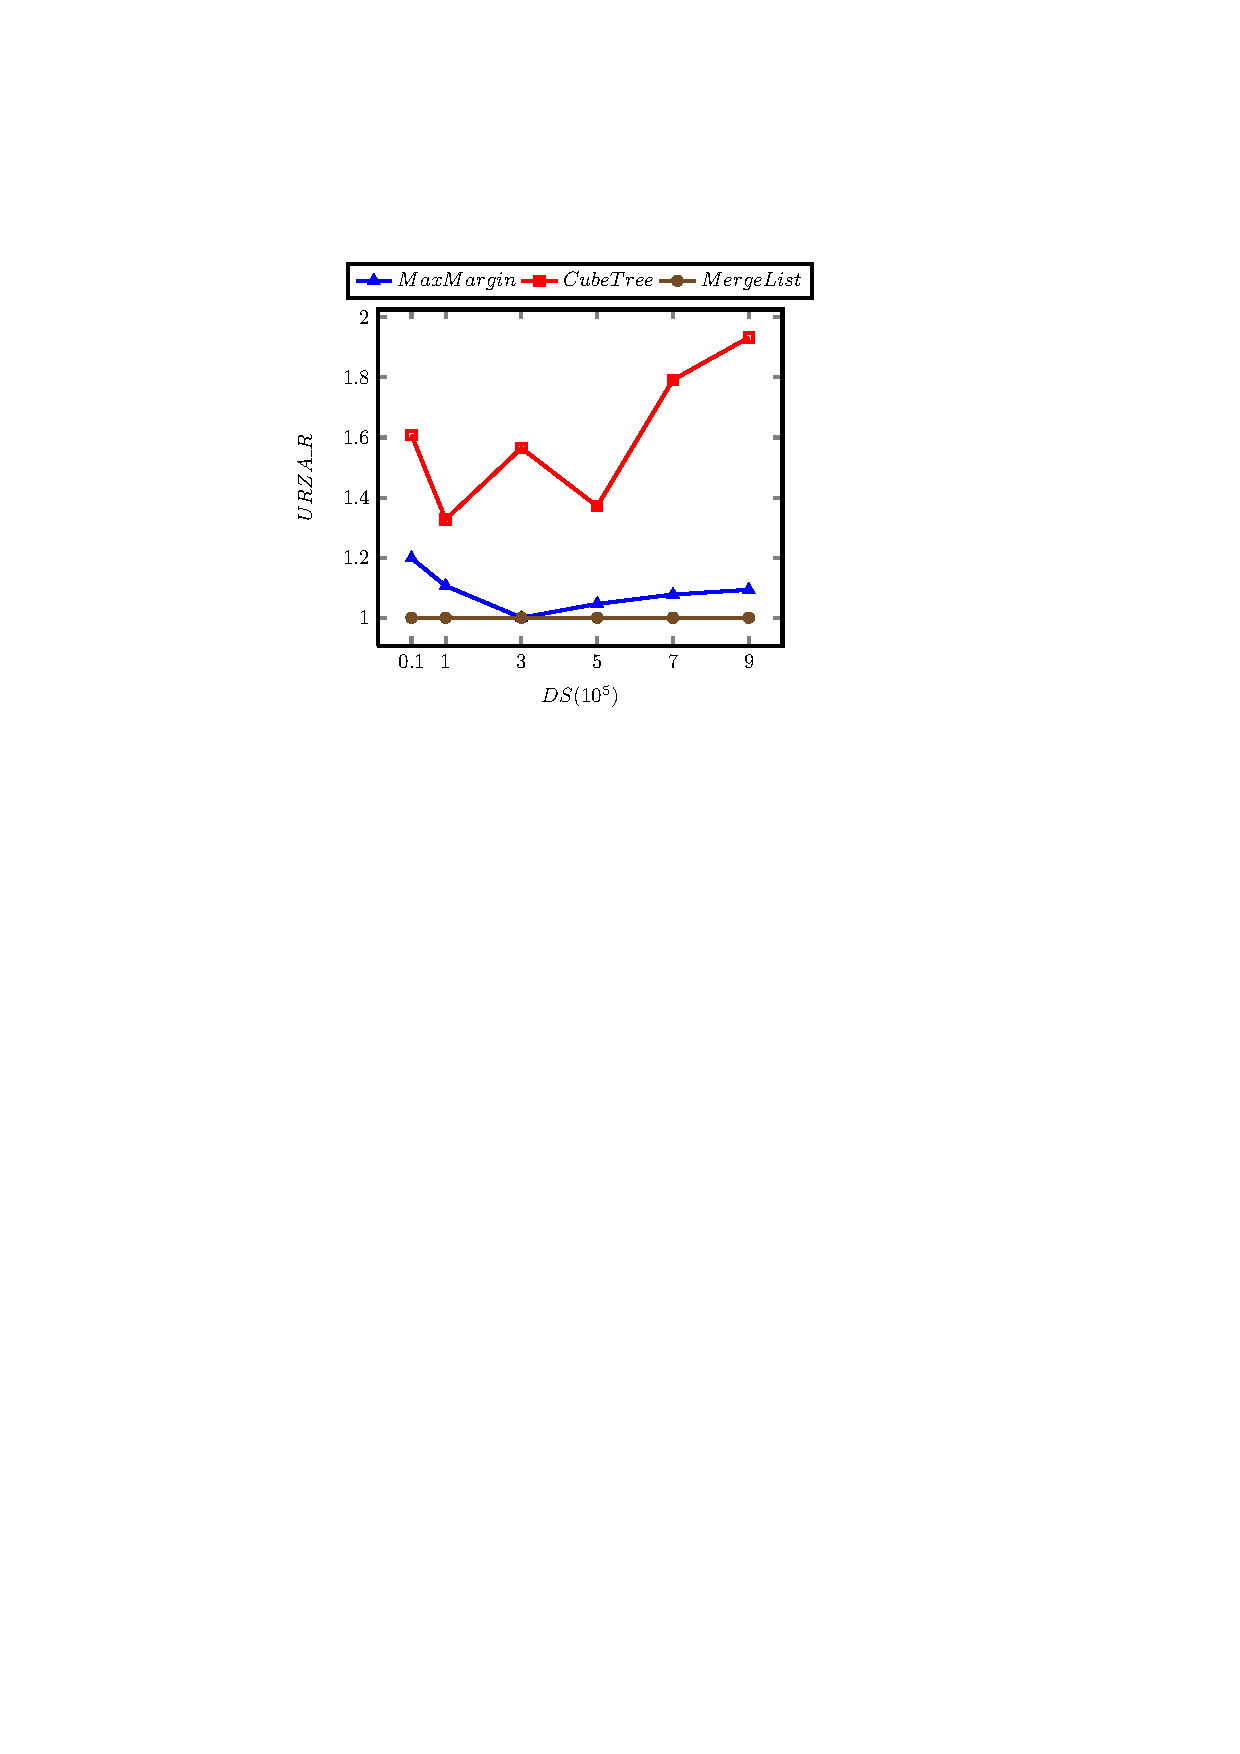
\includegraphics[width=1.5in,height=1.5in]{DS-R}
    }
\caption{Varying the factor DS}
\label{F5}
\end{figure}

\textbf{\textit{Varying the factor DS}}. Figs. \ref{F5}a and \ref{F5}b show the response time and approximation ratio of three algorithms respectively, when we vary the value of DS. We vary the value of DS from 10,000 to 900,000. As expected, as DS increases, the response time of all three algorithms increase. However, as shown in the Fig. \ref{F5}a, the response time of MergeList does not increase dramatically as DS is increased. This is due to the two pruning strategies Lemma 3 and Lemma 4 employed in MergeList. Specifically, although CubeTree runs faster than MaxMargin but the response time of MaxMargin increases slowly than CubeTree in that the merge phase takes much time when DS increases, which reflects that MaxMargin is more adaptive to DS than CubeTree. Fig. \ref{F5}b shows MaxMargin achieves an approximation ratio from 1.0 to 1.2 when we vary DS from 10,000 to 900,000. Especially, the approximation ratio equals to 1 when DS takes the value of 300,000. The approximation ratio of CubeTree with an upper bound 2.0, however, it is unstable.

\begin{figure}[h] \centering
    \subfigure[] { \label{QKa}
    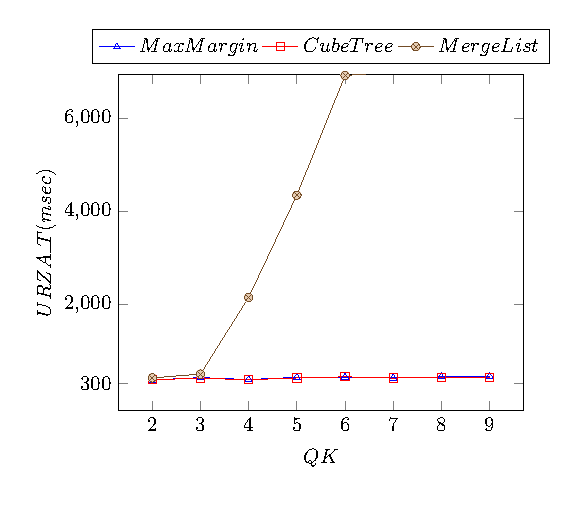
\includegraphics[width=1.5in,height=1.5in]{QK-T}
    }
    \subfigure[] { \label{QKb}
    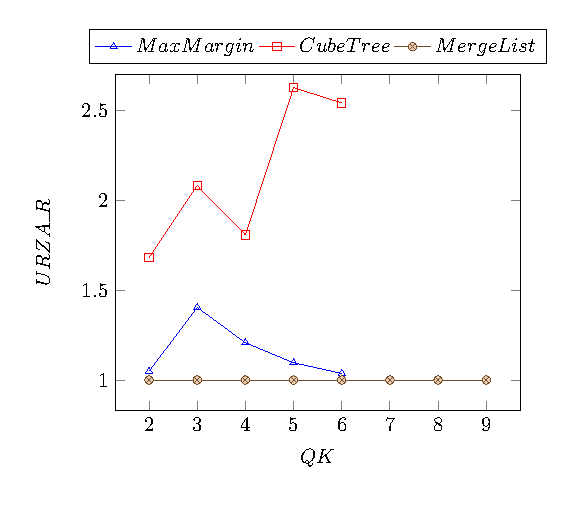
\includegraphics[width=1.5in,height=1.5in]{QK-R}
    }
\caption{Varying the factor QK}
\label{F6}
\end{figure}

\textbf{\textit{Varying the factor QK}}. Figs. \ref{F6}a and \ref{F6}b show the response time and approximation ratio of three algorithms respectively, when we vary the value of QK. In this experiment, we vary the value of QK from 2 to 9. We omit the experiment results when MergeList runs out of memory (e.g., we omit the response time of MergeList in Fig. \ref{F6}a when QK takes the value of 7, 8 and 9, in that it runs out of memory). As shown in Fig. \ref{F6}a, MaxMargin and CubeTree run faster than MergeList. Usually, they are 7-20 times faster than MergeList and their response times are almost not affected by QK as shown in Fig. \ref{F6}a. This is because that with the KHT index, CubeTree can merge the cubeTree nodes efficiently and MaxMargin can select the optimal object from KMPQ directly. Since the exact algorithm MergeList fails to return the optimal solution when QK takes value of 7, 8 and 9, to maintain the integrity of the experiment result curve, for approximation algorithm CubeTree and MaxMargin, we take the average value of existing approximation ratio as the default value. We present these values with the dotted line in Fig. \ref{F6}b. These strategies used in this part also be used in subsequent experiments. As can be observed from Fig. \ref{F6}b, MaxMargin still achieves a better accuracy than CubeTree.

\begin{figure}[h] \centering
    \subfigure[] { \label{KDa}
    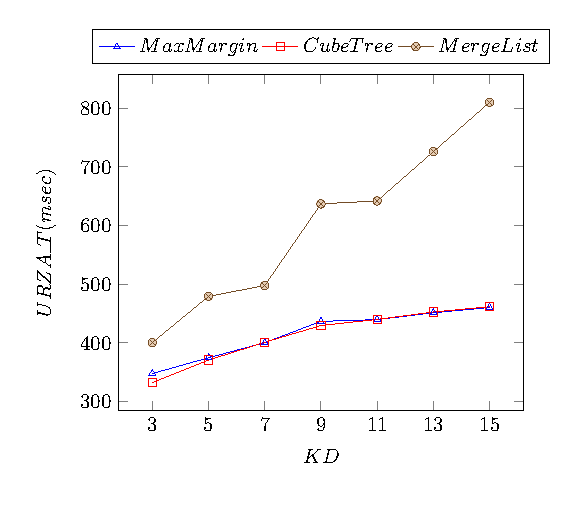
\includegraphics[width=1.5in,height=1.5in]{KD-T}
    }
    \subfigure[] { \label{KDb}
    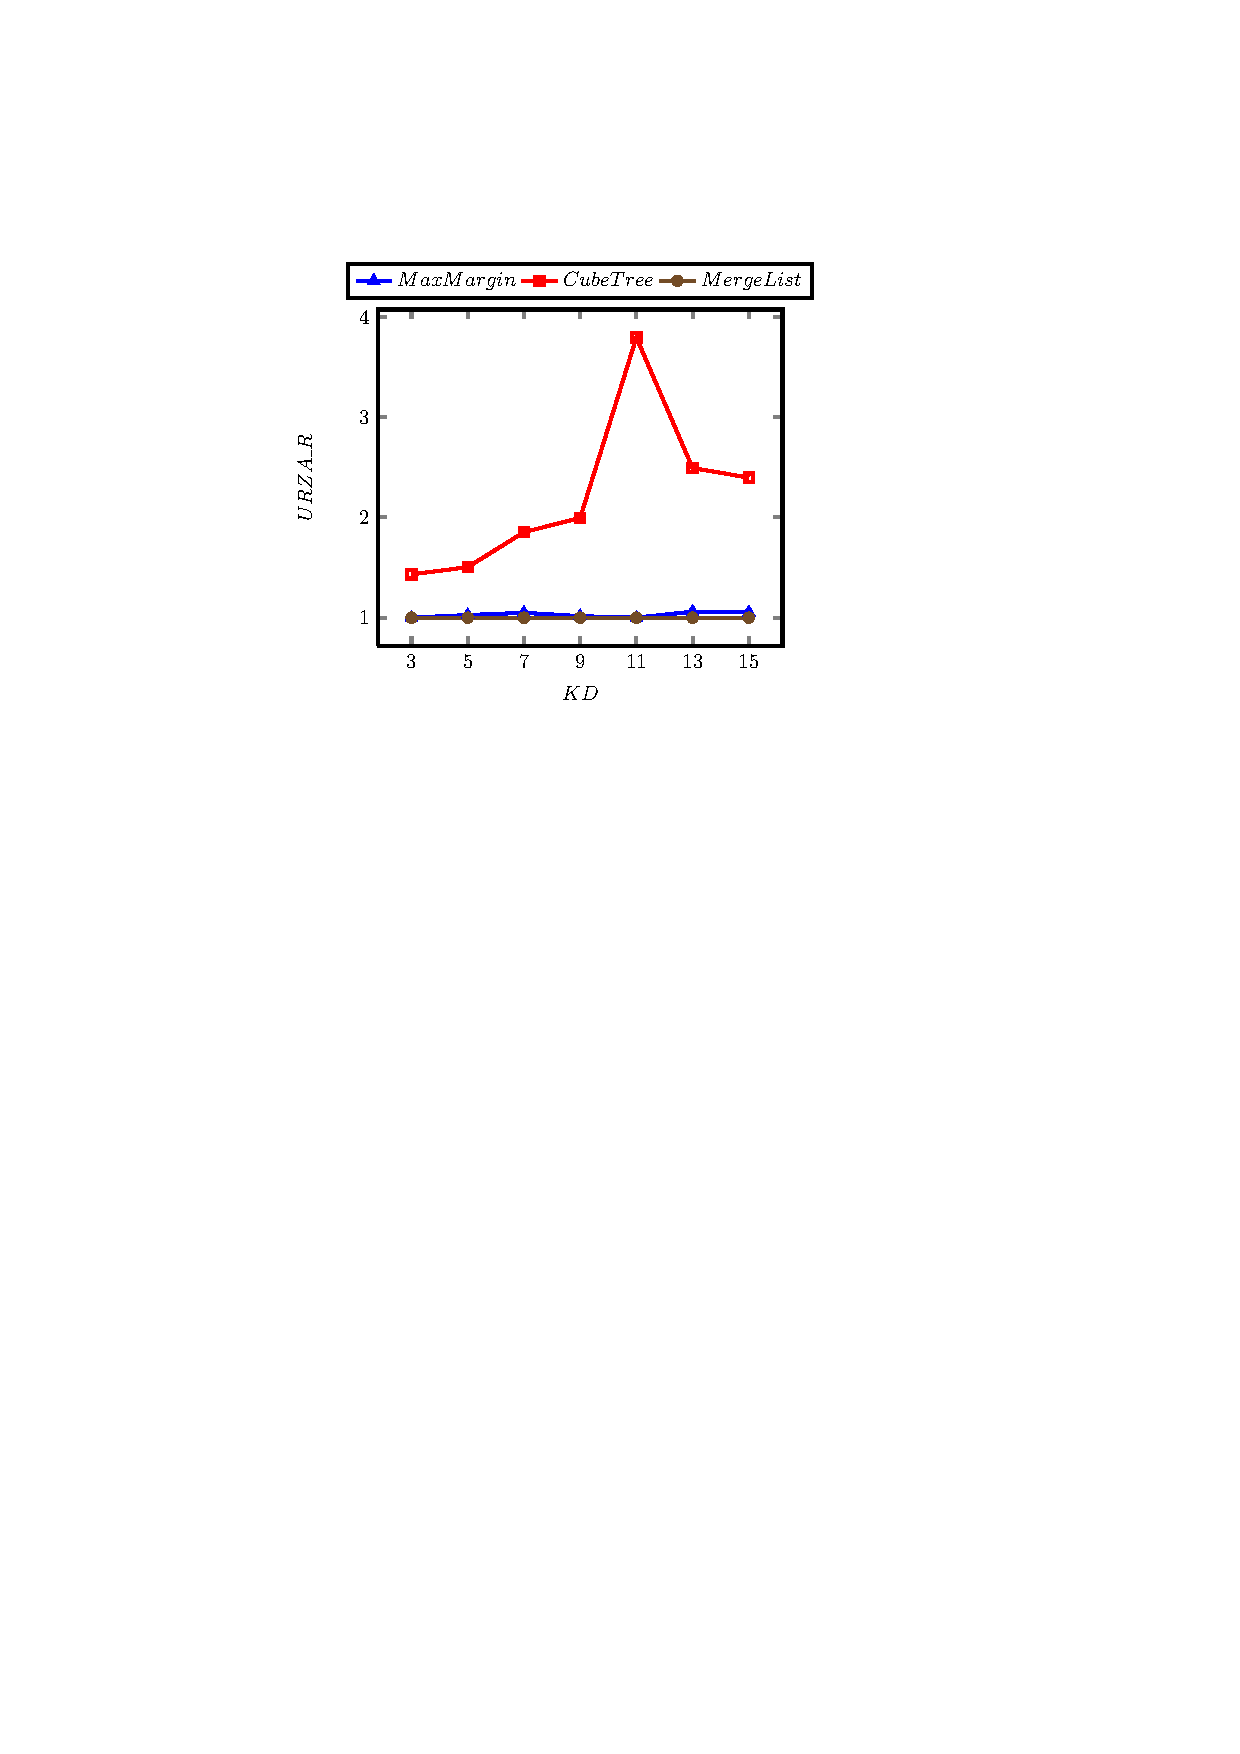
\includegraphics[width=1.5in,height=1.5in]{KD-R}
    }
\caption{Varying the factor KD}
\label{F7}
\end{figure}

\textbf{\textit{Varying the factor KD}}. Figs. \ref{F7}a and \ref{F7}b show the response time and approximation ratio of three algorithms respectively, when we vary the value of KD. Differing with the method in \cite{zhang2009keyword}, which fixes the number of keywords associated with objects, in this set of experiments, we set the upper bound for it by KD. For each object, k keywords are generated, where k is a random positive integer less than the upper bound. We vary KD from 3 to 15. It is shown that MaxMargin and CubeTree run much faster than MergeList as the increases of KD. Specifically, we notice that the response time of all three algorithms increases as KD becomes larger. This is because that the number of relevant objects increases as KD increases. Fig. \ref{F7}b shows that the approximation ratio of MaxMargin changes slightly and is extremely close to 1. In contrast, CubeTree performs the worst in terms of accuracy and stability.

\begin{figure}[h] \centering
    \subfigure[] { \label{TSa}
    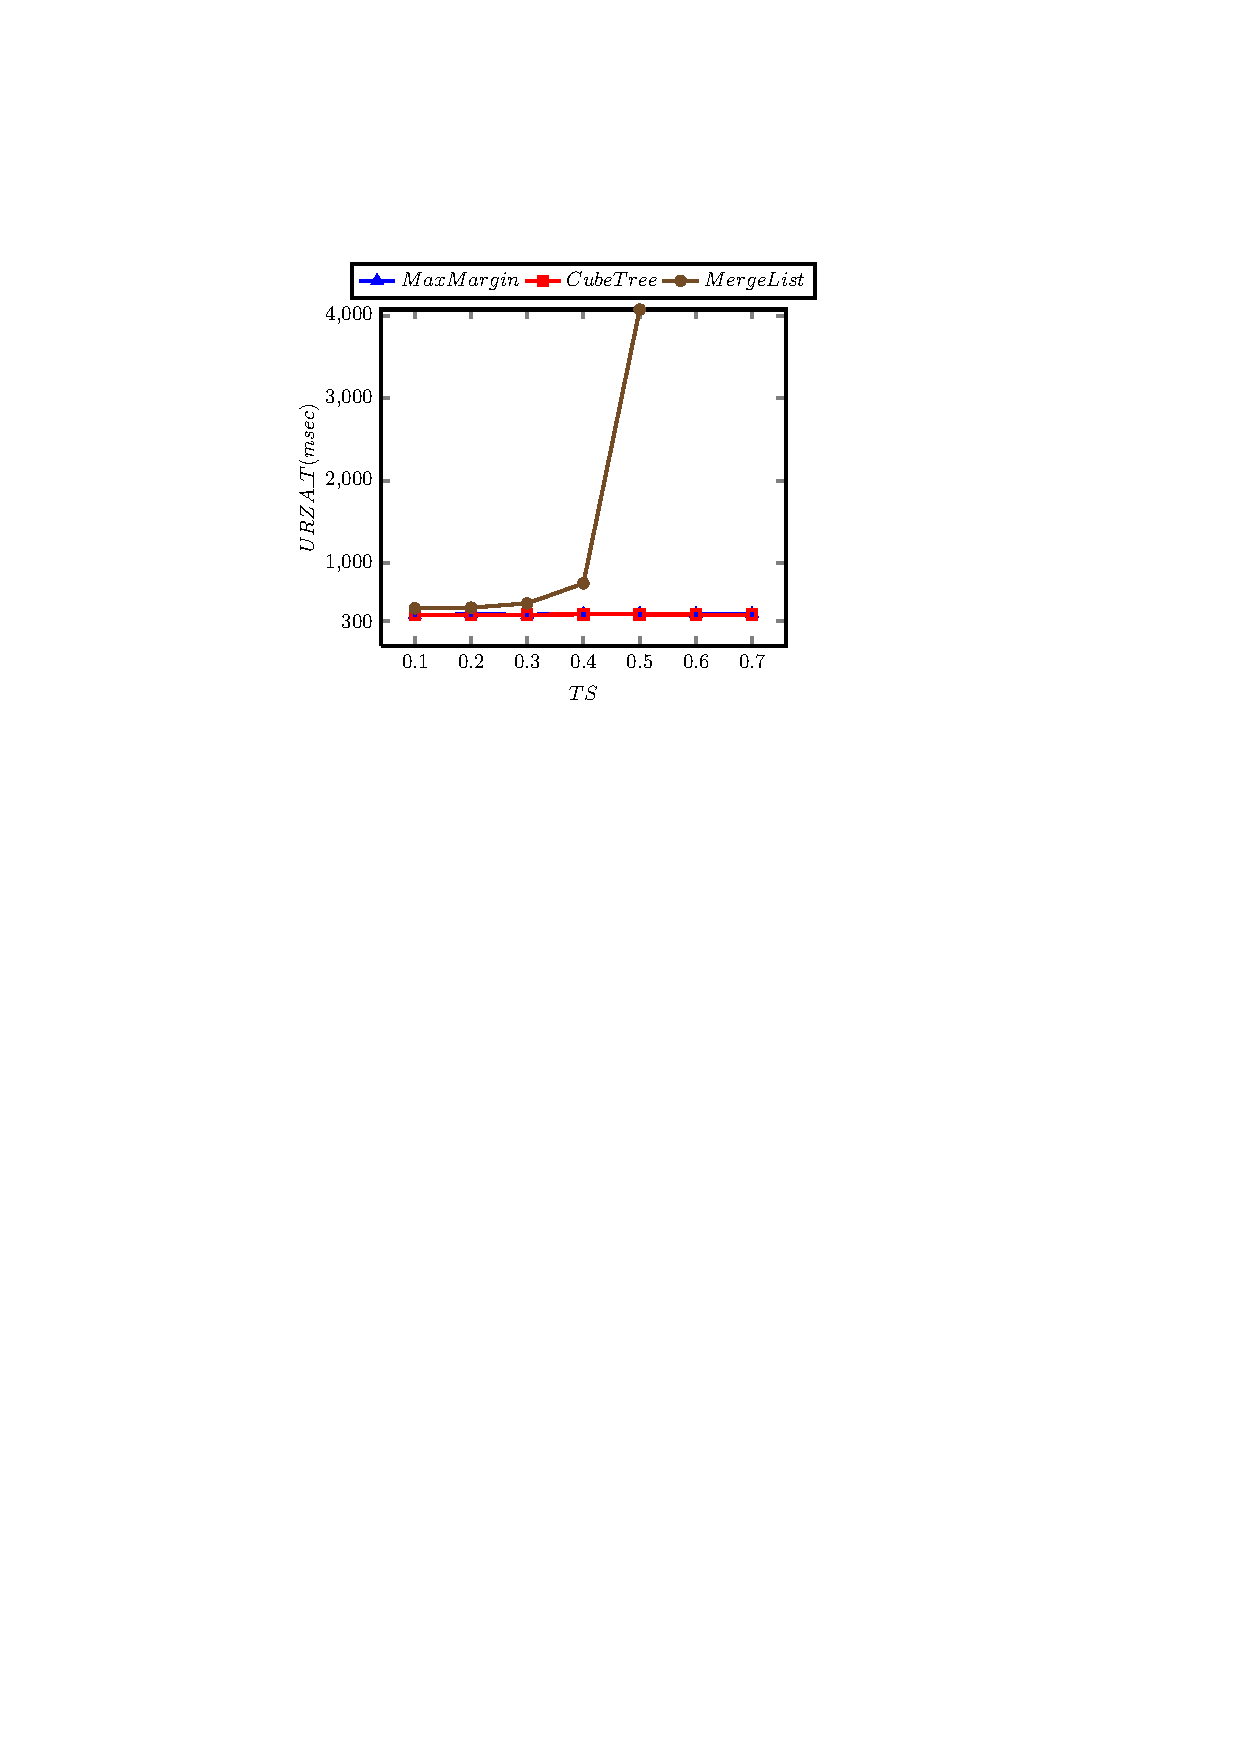
\includegraphics[width=1.5in,height=1.5in]{TS-T}
    }
    \subfigure[] { \label{TSb}
    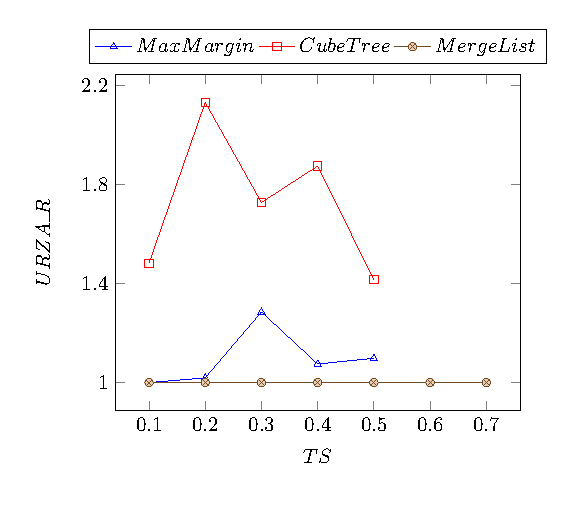
\includegraphics[width=1.5in,height=1.5in]{TS-R}
    }
\caption{Varying the factor TS}
\label{F8}
\end{figure}

\textbf{\textit{Varying the factor TS}}. Figs. \ref{F8}a and \ref{F8}b show the response time and approximation ratio of three algorithms respectively, when we vary the value of TS. The value of TS determines the size of result set, besides, we can obtain the different combinations of object by adjusting TS. In this set of experiments, we vary TS from 0.1 to 0.7. As can be seen from Fig. \ref{F8}a that the response time of MergeList increases dramatically. Especially, MergeList runs out of memory when TS takes the value of 0.6. In contrast, CubeTree and MaxMargin are more adaptive to TS and almost not affected by TS as shown in Fig. \ref{F8}a. This is consistent with earlier findings when we study on the factor of QK. And can be explained with the same reason. Fig. \ref{F8}b shows again, that MaxMargin performs better than CubeTree in terms of approximation ratio.


\begin{figure}[h] \centering
    \subfigure[] { \label{CubeTree-T}
    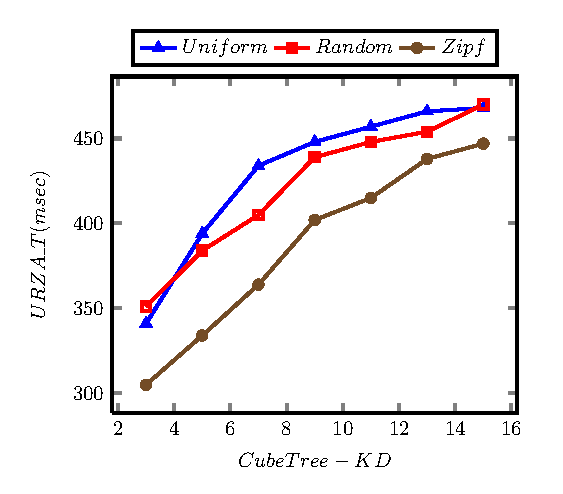
\includegraphics[width=1.5in,height=1.5in]{CubeTree-T}
    }
    \subfigure[] { \label{MaxMargin-T}
    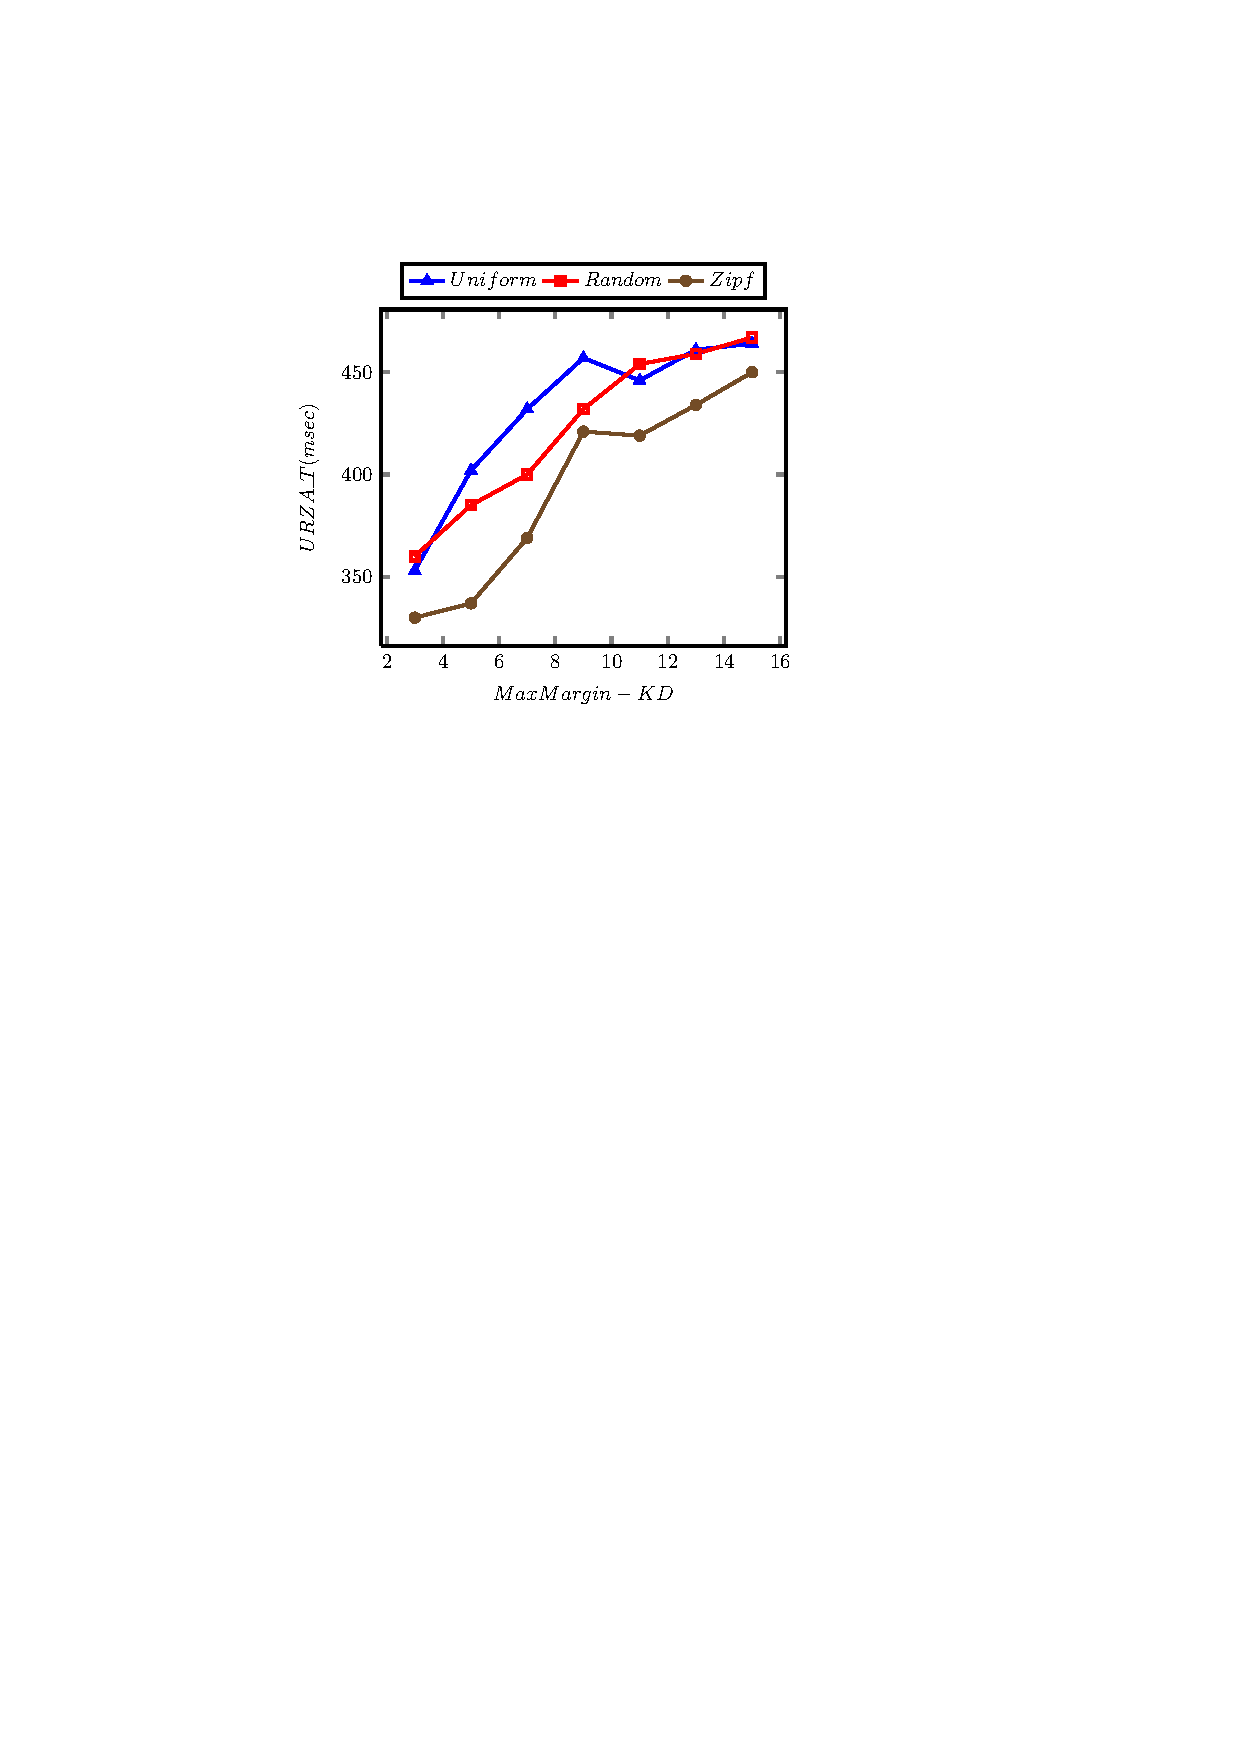
\includegraphics[width=1.5in,height=1.5in]{MaxMargin-T}
    }
    \subfigure[] { \label{MergeList-T}
    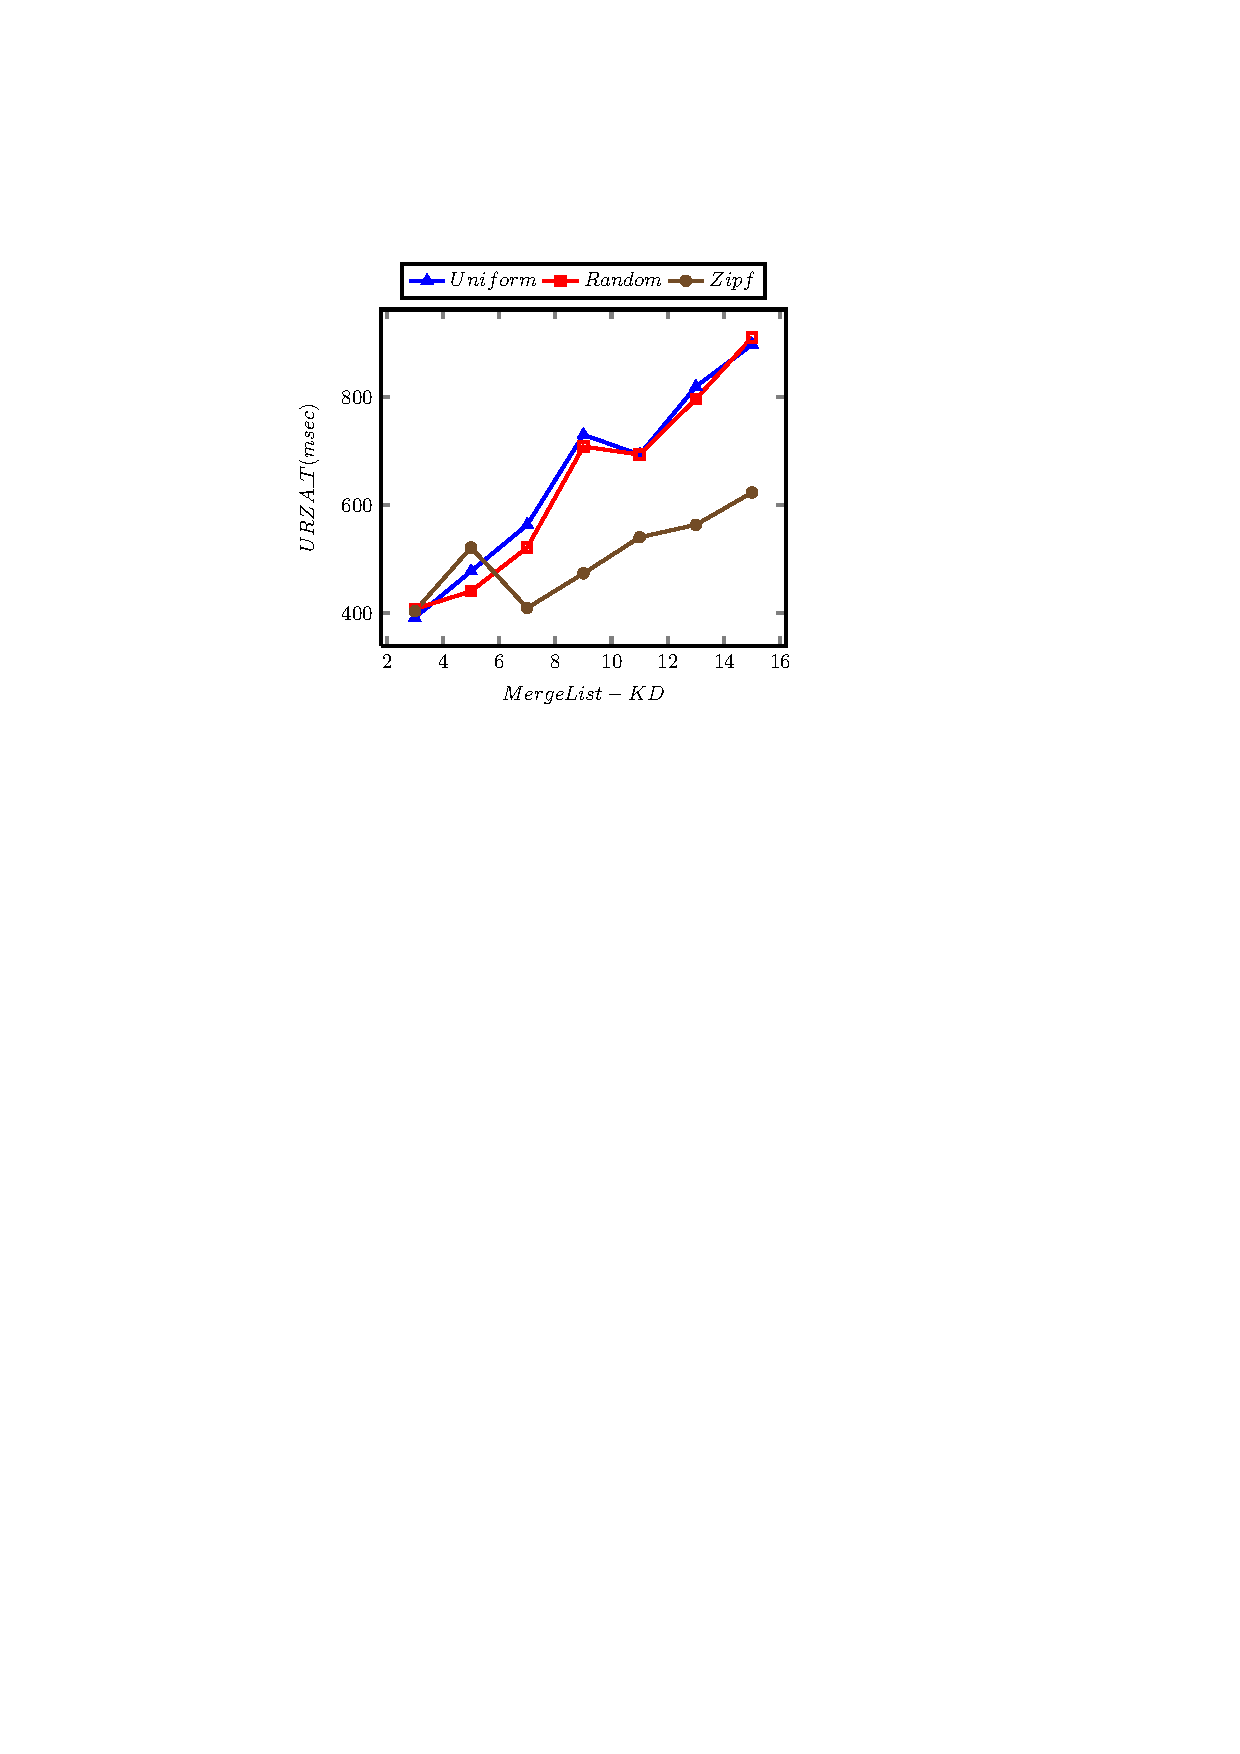
\includegraphics[width=1.5in,height=1.5in]{MergeList-T}
    }
\caption{The Response Time on Different Datasets}
\label{F11}
\end{figure}

\begin{figure}[!ht] \centering
    \subfigure[] { \label{CubeTree-R}
    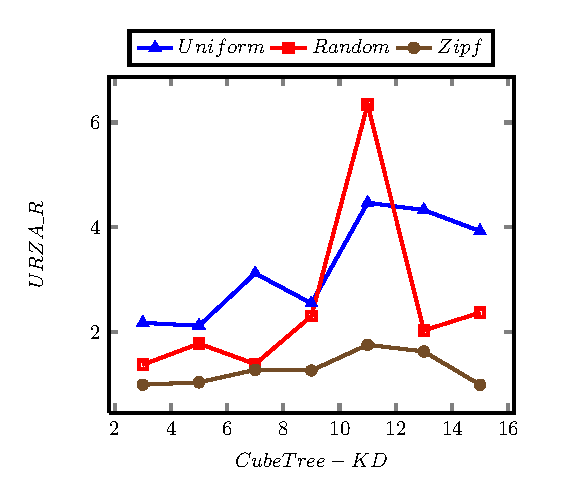
\includegraphics[width=1.5in,height=1.5in]{CubeTree-R}
    }
    \subfigure[] { \label{MaxMargin-R}
    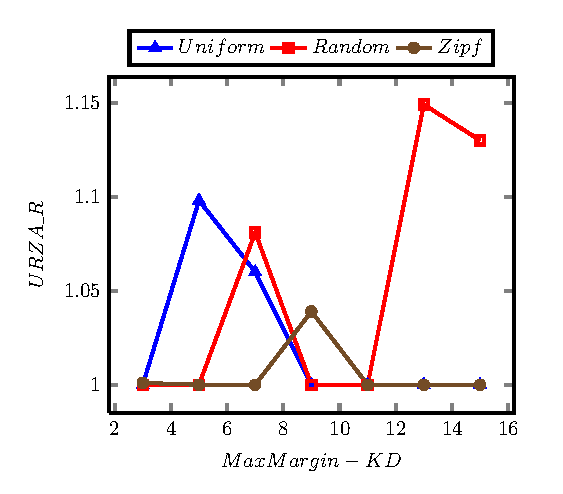
\includegraphics[width=1.5in,height=1.5in]{MaxMargin-R}
    }
    \subfigure[] { \label{MergeList-R}
    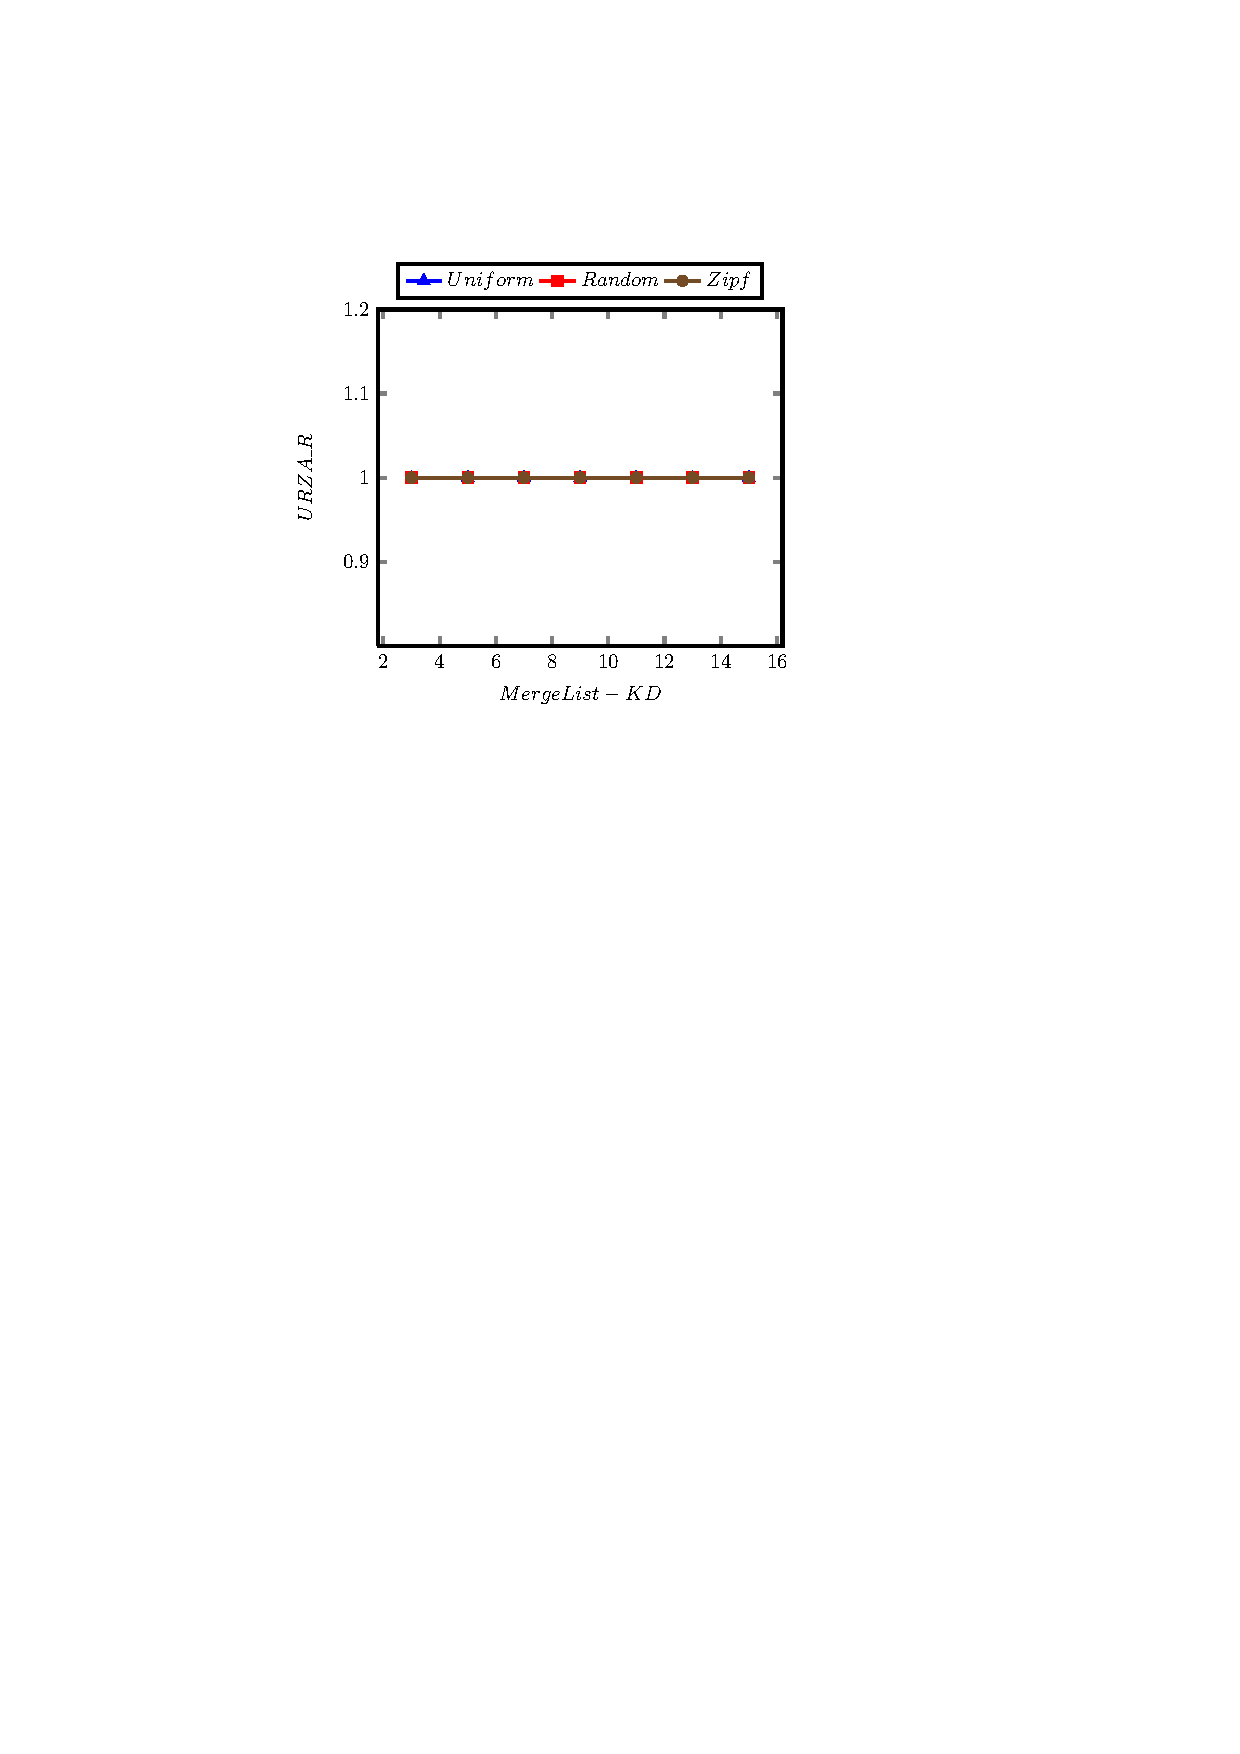
\includegraphics[width=1.5in,height=1.5in]{MergeList-R}
    }
\caption{The Approximation Ratio on Different Datasets}
\label{F12}
\end{figure}

\textbf{\textit{The performance on Different Datasets.}} To further illustrate the performance of our algorithms on different types of datasets. In this set of experiments, we study the performance of our proposed algorithms on different datasets from the aspect of KD. Figs. \ref{F11} and \ref{F12} show the response time and approximation ratio of our algorithms on different datasets, respectively. Specifically, Figs. \ref{F11}a, \ref{F11}b and \ref{F11}c illustrate the response time of CubeTree, MaxMargin and MergeList respectively. Curves in figures correspond to three datasets, namely, uniform, random and zipf. As can be observed from Fig. \ref{F11}, that all algorithms are adaptive to zipf dataset. And performance on random dataset is better than on uniform dataset. These phenomenons could be partially attributed to the effect of data skew, which affects the number of relevant objects. Figs. \ref{F12}a, \ref{F12}b and \ref{F12}c illustrate the approximation ratio of CubeTree, MaxMargin and MergeList respectively. And curves in figures correspond to three datasets, namely, uniform, random and zipf. We notice that all algorithms achieve better accuracy on zipf dataset than other two datasets. And uniform dataset performs better than random dataset in terms of accuracy and stability. In a nutshell, all three algorithms perform well on zipf dataset in both response time and approximation ratio. Random dataset with better performance on response time, but worse stability on accuracy than uniform dataset on three algorithms.

\begin{table}[!hb]
\centering
\begin{tabular}{|l|l|}
\hline
Items Of CA & The Scale Of Items \\
\hline
Number of objects (or keywords) & 2761823 \\
\hline
Number of unique keywords & 63 \\
\hline
Number of combined objects & 20694 \\
\hline
\end{tabular}
\caption{The real data of CA}
\label{T5}
\end{table}

\subsection{Results on Real Dataset}
In this section, we mainly study the response time and approximation ratio of our proposed algorithms on real data set CA, which was collected from the U.S. Board on Geographic Names(geonames.usgs.gov).
\begin{figure} \centering
    \subfigure[] { \label{RQKa}
    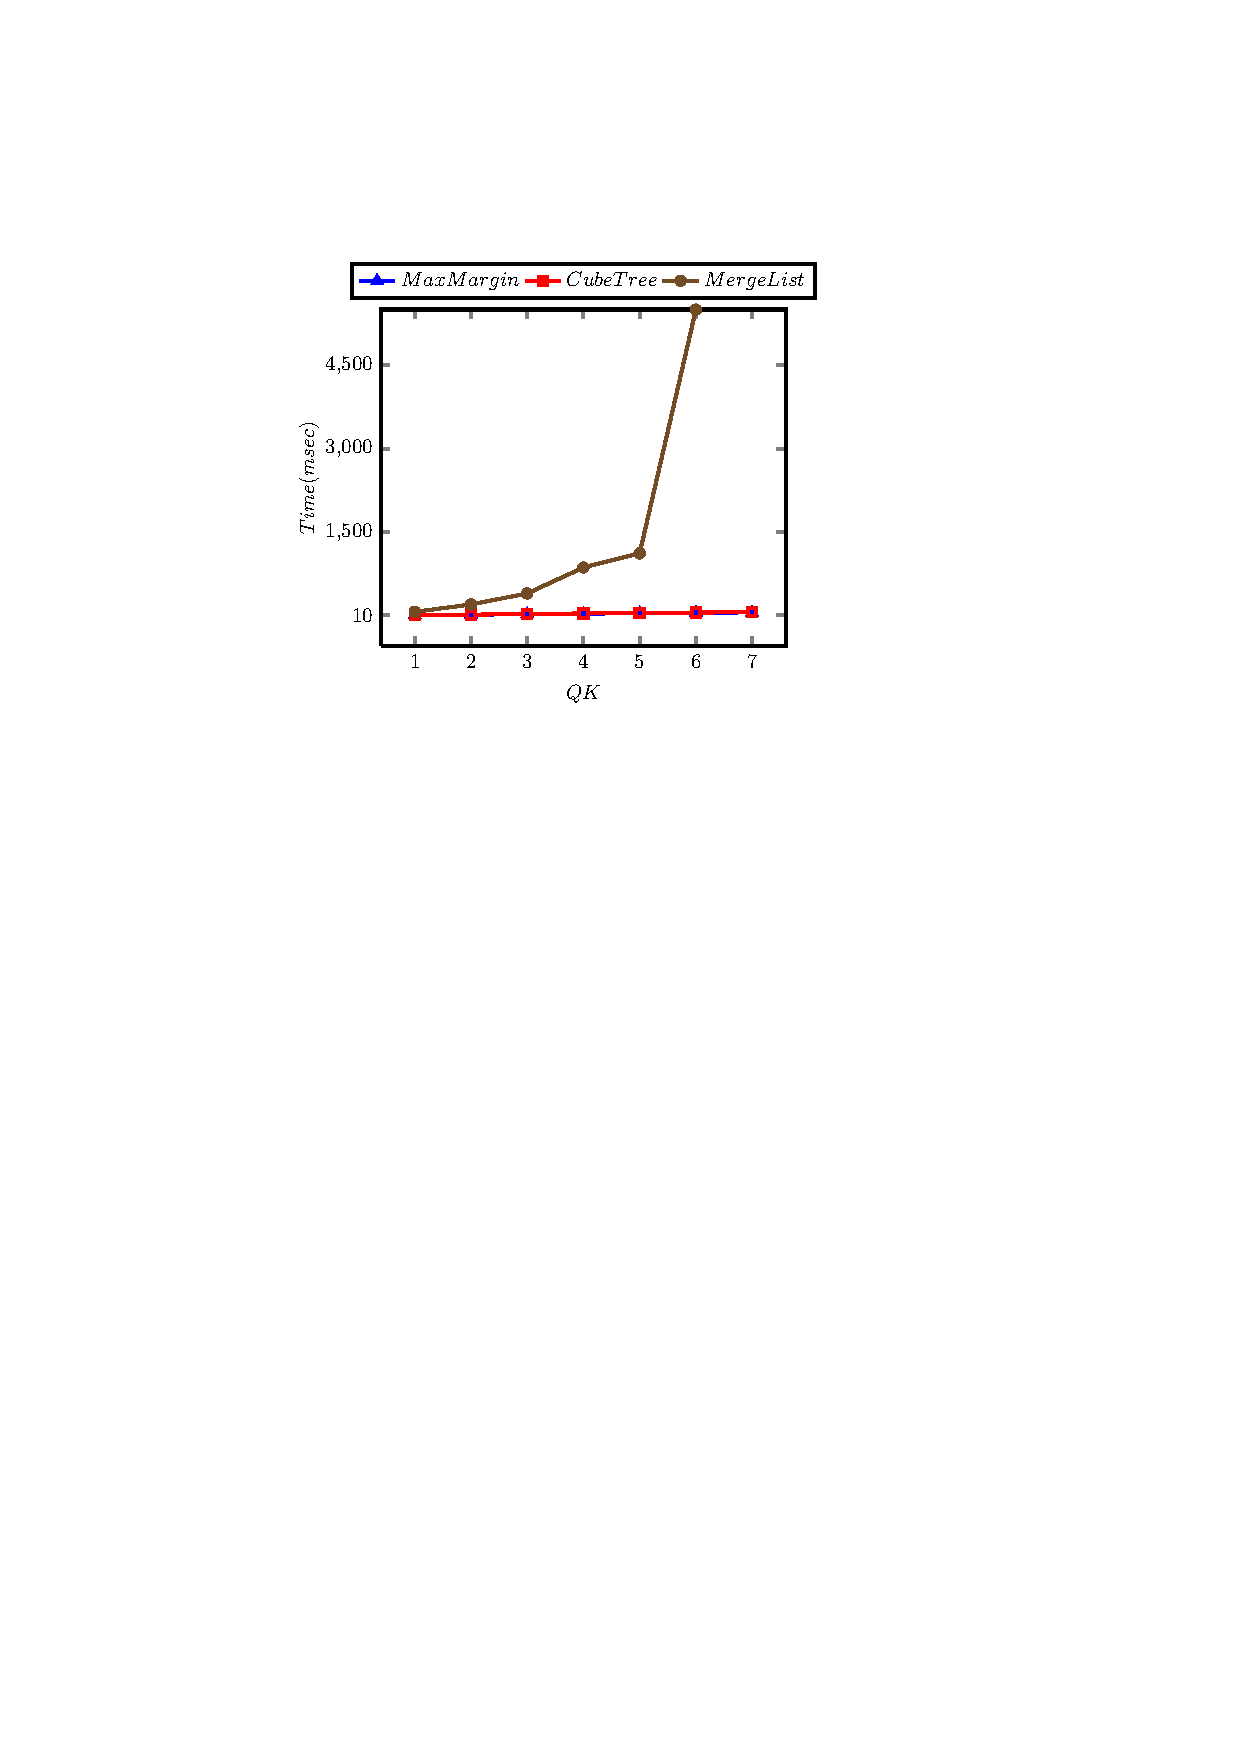
\includegraphics[width=1.5in,height=1.5in]{RQK-T}
    }
    \subfigure[] { \label{RQKb}
    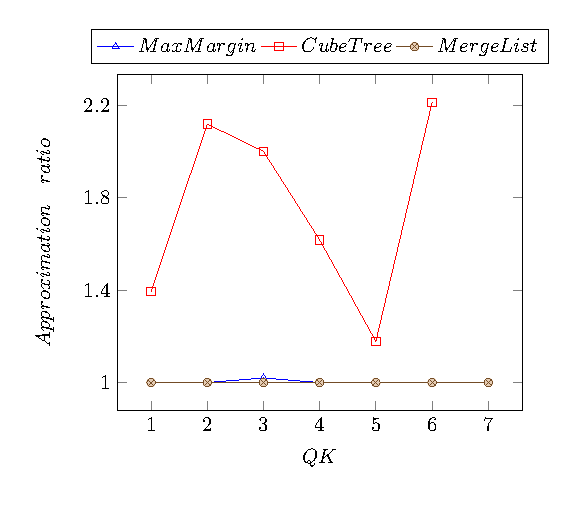
\includegraphics[width=1.5in,height=1.5in]{RQK-R}
    }
\caption{Varying the factor QK}
\label{F9}
\end{figure}

\begin{figure}[h] \centering
    \subfigure[] { \label{RTSa}
    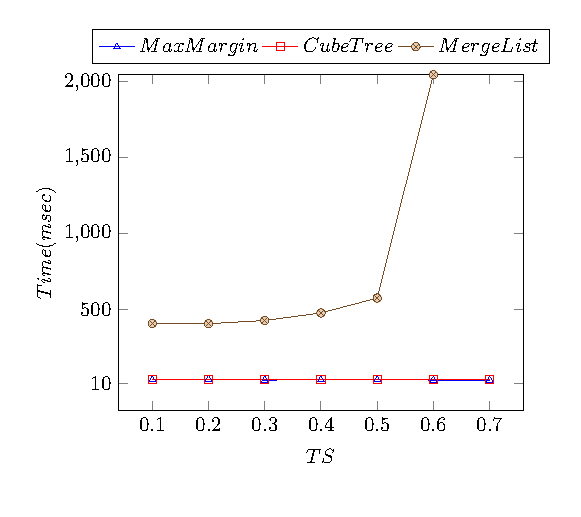
\includegraphics[width=1.5in,height=1.5in]{RTS-T}
    }
    \subfigure[] { \label{RTSb}
    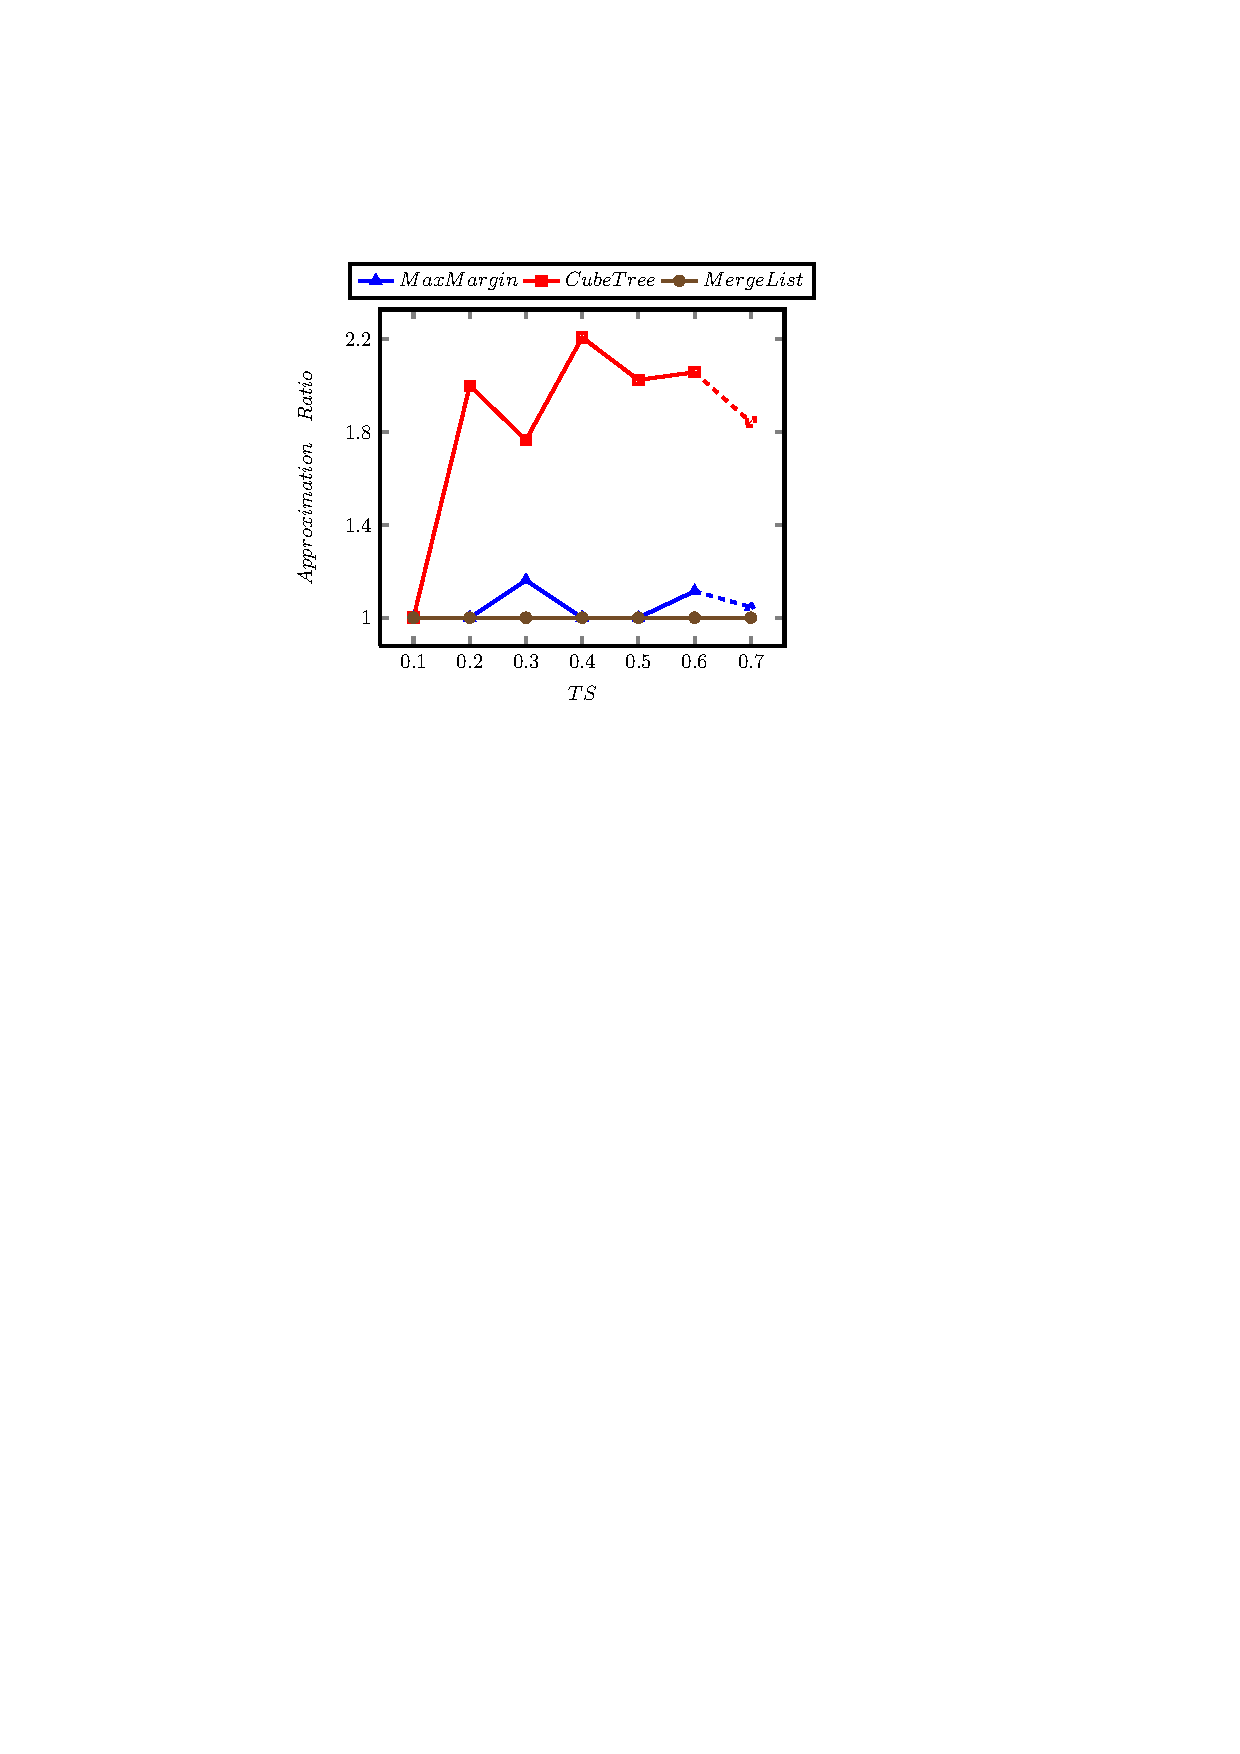
\includegraphics[width=1.5in,height=1.5in]{RTS-R}
    }
\caption{Varying the factor TS}
\label{F10}
\end{figure}

Each object of Geographic Names is a 2D location associated with a set of items describing it (e.g., a geographic name like Locate). We use the \textit{feature class} (e.g., School and Hospital) as the keyword. Since there is only one single feature class associated with each object, which is different from our assumption that each object is associated with several keywords. To address this problem, we associate object o with keywords obtained by aggregating the feature class of all objects whose distance to o within a given threshold. Finally, we obtain 20,694 objects in total as shown in Table \ref{T5}. And we assign an integer number (e.g., 1,2,3,4,5) randomly for it as the level information, an integer number ranges from 1 to 100 as the cost of o.

Since factors of TK, DS and KD are fixed for CA dataset. We study the effect of QK and TS on real dataset. Figs. \ref{F9} and \ref{F10} show the experiment results of QK and TS, respectively. As can be observed from Fig. \ref{F9}a that MergeList runs out of memory when QK takes the value of 7, and both CubeTree and MaxMargin almost not be affected by QK, which is consistent with the observations in Fig. \ref{F6}a. Fig. \ref{F9}b shows that the solution of MaxMargin extremely approaches to optimal solution. However, the accuracy of CubeTree is unstable. Fig. \ref{F10} shows the performance of our algorithms when we vary TS from 0.1 to 0.7, as shown in Fig. \ref{F10}, the performance is consistent with the observations in Fig. \ref{F8}.

From the comprehensive experiments on both synthetic and real-life datasets, we can see that, both CubeTree and MaxMargin run much faster than the exact algorithm MergeList. CubeTree runs slightly faster than MaxMargin, however, MaxMargin with better performance than CubeTree in terms of accuracy and stability of approximation ratio. 


\section{Conclusions and Future Work}
%CONCLUSIONS AND FUTURE WORK
In this paper, we introduce and solve a novel type of queries, namely, KaGWC query. Although CoSKQ can retrieve a group of objects to collectively satisfy the users' needs, however, these exsiting works regardless of the crucial level information of keyword. BKC \cite{deng2015best} considers the rating information, but different with ours in query goal. To address this novel problem, we design two approximation algorithms, namely, CubeTree and MaxMargin with provable approximation ratio. Besides, we also propose an exact algorithm MergeList for this problem. Extensive experiments on both real and synthetic datasets were conducted to verify the performance of our proposed algorithms. In a nutshell, both CubeTree and MaxMargin run much faster than the MergeList. CubeTree runs slightly faster than MaxMargin, however, MaxMargin with better performance than CubeTree in terms of accuracy and stability of approximation ratio.

In the future work, there are several interesting research directions. One is to research the KaGWC problem in the road network scenario. Another direction is to take multidimensional level information of keyword into consideration, which can provide the user more appropriate query result. It is also interesting to study other forms of cost function for this problem.


\textbf{Acknowledgements:} This work was supported in part by the National Key Technology Support Program Grants 2012BAH03F02 and 2013BAH62F01, NSFC Grant 61379033, the Fundamental Research Funds for the Central Universities under Grant 2013QNA5020, Zhejiang Province Funds for Science and Technology Innovation Team Grant 2010R50040, and the Key Project of Zhejiang University Excellent Young Teacher Fund (Zijin Plan).

%\section{REFERENCES}
%%REFERENCES
\bibliographystyle{abbrv}
\bibliography{kwd}
\end{document}
